\documentclass{article}
\usepackage[utf8]{inputenc}
\usepackage{comment}
\usepackage{duomasterforside}
\usepackage{listings}
\usepackage{float}
\usepackage{fancyvrb}
\usepackage{xcolor}
\usepackage{fvextra}
\usepackage{soul}
\usepackage{minted}
\graphicspath{ {./graphics/} }
\usepackage[backend=biber,natbib,style=numeric]{biblatex}
\usepackage{hyperref}
\addbibresource{references.bib}


\begin{document}

\title{Mobile Assets in Semantic Digital Twins}
\author{Oscar Lund Ramstad}
\date{January 2023}

\duoforside[dept={Institute for Informatics}, program={Informatics: Programming and System Architecture}, short]

\section*{Abstract}


\newpage

\section*{Acknowledgements}
\newpage

\tableofcontents
\newpage

\listoftables
\newpage

\listoffigures
\newpage

\pagenumbering{arabic}
\setcounter{page}{1}

\section{Introduction}\label{sec:Introduction}
\subsection{Context}
A digital twin (DT) is a digital representation of some physical system, referred to as a physical twin (PT), that is twinned in near real-time by the DT in order to understand or control the PT \cite{grieves_digital_2017, kamburjan_digital_2022}. The twinning aims to be bidirectional meaning that the DT both observes the PT and communicates informed decisions back to it \cite{kamburjan_digital_2022, fuller_digital_2020}. The DT must continually adapt to correctly reflect its physical twin \cite{kamburjan_twinning-by-construction_2022}. This may pose a challenge if the PT contains mobile assets, such as smartphones. The number of smartphone users worldwide is at an all-time high \cite{petroc_taylor_number_2023}. They are important resources for a company and can change at any time \cite{marcheta_development_2022}.

There exist challenges in handling mobile assets. Some systems mainly focus on tracking mobile assets and the accuracy of their physical location \cite{marcheta_development_2022,akram_design_2021}. If we keep the company's assets in mind, such a system could be improved upon by better understanding and controlling asset behavior. 

Furthermore, there is existing research about using Building Information Modeling (BIM) with standard data formats, such as JSON or Resource Description Framework (RDF), to better define static building infrastructure \cite{pauwels_live_2023}. \citeauthor{pauwels_live_2023} proposes how, and to what extent, such data can be used in robot navigation. Although BIM can be used, by default it has some challenges regarding interoperability due to heterogeneous data \cite{dinis_bim_2022,godager_concept_2021}. 

It is stated by \citeauthor{godager_concept_2021} that although BIM could serve as a basis for DTs by providing lots of relevant information, DTs give even more context about the built environment, especially by monitoring assets from near real-time data. A lot of work goes into modeling physical assets in general \cite{waszak_let_2022}, and using BIM is also very costly due to frequent updates by maintainers \cite{hamledari_ifc-based_2018}.

\citeauthor{waszak_let_2022} proposes the use of knowledge graphs (i.e. using graphs to represent data from diverse sources \cite{hogan_introduction_2022, ryen_building_2022}) in the interconnection of various elements in DTs. Instead of storing all related data in one place, they propose storing static and dynamic data sources in different places and linking them.

Handling mobile assets in a DT based on a dynamic asset model (i.e. a file that contains an organized description of an asset's composition and properties \cite{kamburjan_twinning-by-construction_2022} is unexplored territory.


\subsection{Motivation}
Given the gap that exists in connecting tracking systems, asset models, and digital twins, there is still room for improvement. The problem is that there exist no systems that have a digital twin (DT) based on a dynamic asset model which can track an unlimited number of heterogeneous smartphones. In an attempt to formalize heterogeneous data and make it understood by computers, semantic web technologies should be used. More specifically, we aim to semantically enrich a model of a building to increase interoperability, as well as keep it inexpensive and easy to maintain.

We envision a \emph{semantic} digital twin (i.e. a digital twin that processes heterogeneous data from different sources in the domain into generally understandable information \cite{birgit_boss_digital_nodate}) based on a dynamic asset model in which static data (existing building infrastructure) and dynamic data (smartphone's physical location) is separated. The DT will be able to track an unlimited number of mobile assets simultaneously. The DT will be formalized using semantic web technologies. In the knowledge graph, static data will be noted to be different than dynamic data as it is generated from a combination of the program state and the asset model. 

The asset model will be automatically reloaded by the system itself, or manually updated by an operator either offline (online version updated from local changes), or directly online in an ontology editor. This way the mobile assets are not only tracked, but the physical system containing them is twinned in near-real time as well. The DT will get positional sensor data from the PT, and then send informed decisions back to the PT.

\subsection{Problem statement}
From the context of digital twins and an increasing number of smartphone users, as well as the motivation for improvement, we present the following hypothesis (H):

\begin{itemize}
    \item[\textbf{H:}] We can handle mobile assets in a semantic digital twin with the use of a dynamic asset model of a simple building, in which dynamic data (smartphone's physical location) is automatically updated by a server and separated from static data (existing building infrastructure), and informed decisions are sent back to the physical twin.
\end{itemize}


In addition to this, we present the following three research questions which will guide this thesis:
\begin{itemize}
    \item[\textbf{RQ1:}]
    Can we create a dynamic asset model of a simple building that is also extensible?
    \item [\textbf{RQ2:}] 
    Can we enable bidirectional data flow between the PT and DT, such that the digital twin gets updated sensor data from mobile devices and sends informed decisions back?
    \item [\textbf{RQ3:}]
    Can we clearly separate dynamic data (smartphone's position) from static data (building infrastructure) in the asset model and in the DT?
\end{itemize}

Having the aforementioned in mind, a possible overview of this thesis' components is shown below in Figure \ref{fig:initial_components}.

\begin{figure}[H]
    \centering
    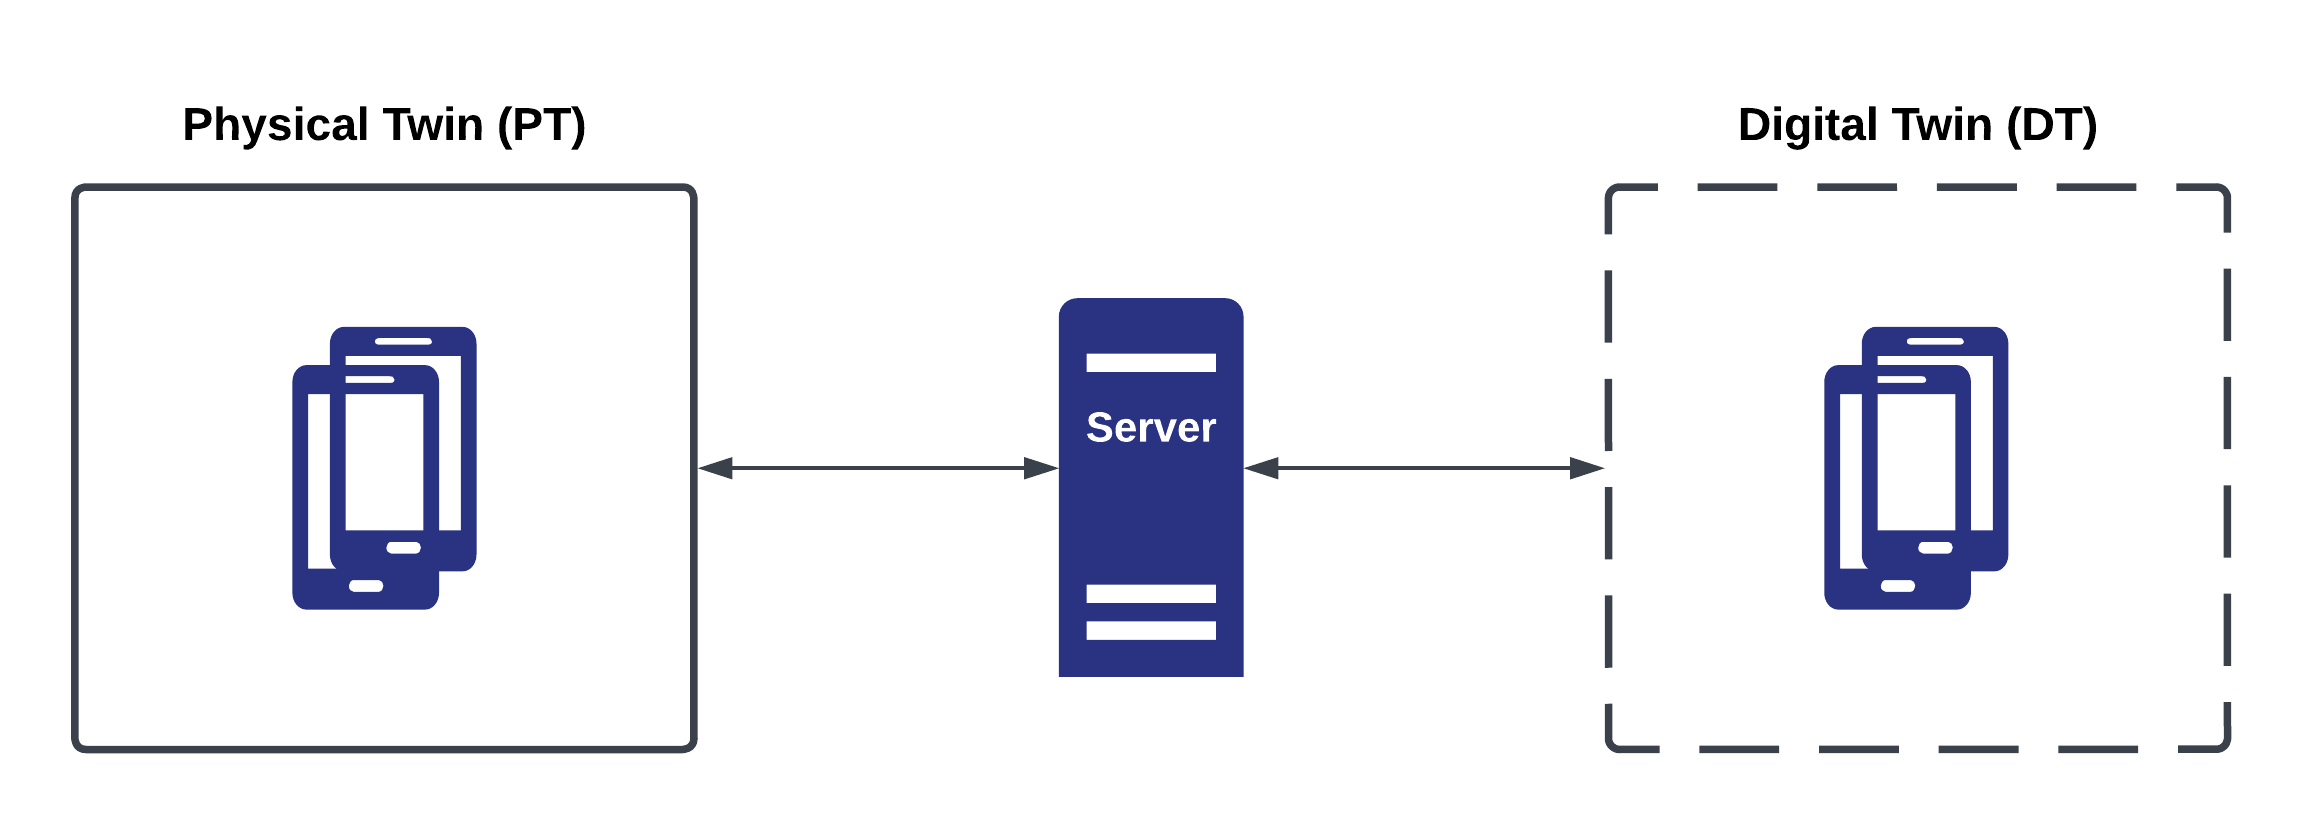
\includegraphics[scale=0.14]{graphics/initial_thesis_overview.png}
    \caption{Possible overview of architectural components in this thesis.}
    \label{fig:initial_components}
\end{figure}


\subsection{Thesis scope and outline}\label{subsec:Scope}
The scope of this thesis is to handle an unlimited number of mobile assets in a semantic digital twin based on a dynamic asset model. Figure \ref{fig:initial_components} shows the possible overview of architectural components and the bidirectional data flow between the PT and DT. The digital twin should be developed using the Semantic Micro Object Language (SMOL) described in \ref{subsec:SMOL}(SMOL) and its publicly available interpreter\footnote{\url{https://github.com/smolang/SemanticObjects}}.

As noted by \citeauthor{pauwels_live_2023} many physical objects, such as furniture and doors, can be movable entities in a building apart from the robots. Doors will have one state (open). Laptops can also be considered mobile assets, but due to the context of a crisis situation, we are not able to justify adding support for it. We limit ourselves to smartphones and tablets in 2D space.  

The areas are predefined squares with latitude and longitude ranges, where we assume the coordinates align. Square areas are easier to compute and scale into larger areas, and we are not concerned with other shapes such as polygons. The analysis of what certain area(s) are (e.g. what does a critical area mean) is also outside the scope of this thesis.

We are also assuming the PT contains a building in which there can be smartphones since we create a digital representation of a building in the DT.

Figure \ref{fig:simple_building} shows a simple building with two rooms connected by an inner wall with a door (open) in it.

\begin{figure}[H]
    \centering
    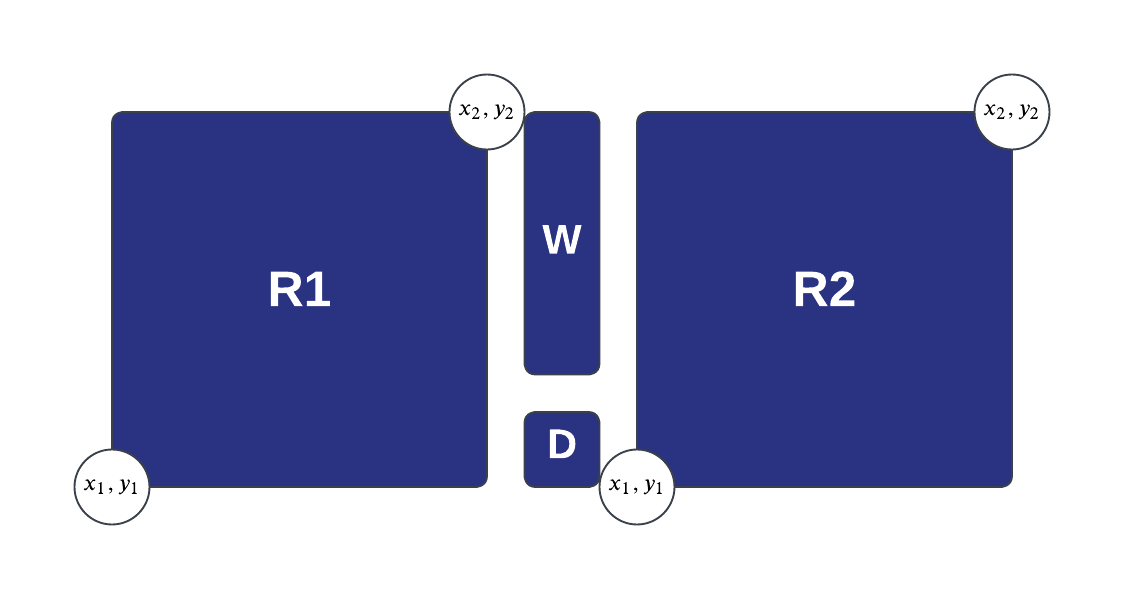
\includegraphics[scale=0.3]{graphics/simple_building.png}
    \caption{A simple building with the structural components: two rooms (R1 and R2) connected by an inner wall (W) with a door (D) in it.}
    \label{fig:simple_building}
\end{figure}


The remainder of this thesis is organized as follows:
\begin{itemize}
    \item \hyperref[sec:Background]{\textbf{Background}} describes the theoretical background of this thesis.
    \item \hyperref[sec:Analysis]{\textbf{Problem analysis and design}} investigates the problem statement and research questions. We also look at what a dynamic asset model means, as well as the separation of static and dynamic data.
    \item \hyperref[sec:Implementation]{\textbf{Implementation}} dives into the implementation of the proposed solution and how the different architectural components shown in Figure \ref{fig:components} interact. More specifically, how do we "close the loop" by sending informed decisions back to the PT. 
    \item \hyperref[sec:Evaluation]{\textbf{Evaluation}} evaluates the proposed solution according to the structural requirements that were set.
    \item \hyperref[sec:Discussion]{\textbf{Discussion}} discusses the discoveries of this thesis and compares them to other existing results and theories. This section also explores the originality of the discoveries.
    \item \hyperref[sec:Conclusion]{\textbf{Conclusion and further work}} concludes this thesis. Mainly we look at the improvements that can be made to the proposed solution in the future.  
\end{itemize}



\newpage
\section{Background}\label{sec:Background}
This section describes the background information of this thesis. Starting off we give an in-depth description of digital twins (DTs). Then we give a description of the vision of a Semantic Web, as well as the technologies that help us build it. Later on we describe semantic reasoning and tools for it.  Then we look at frameworks for building cross-platform applications from a single codebase. Near the end of the section, we describe real-time and time-series databases.

\subsection{Digital Twin}\label{subsec:DigitalTwins}

The \emph{idea} of a digital twin can be traced back to the 1960s in NASA's space exploration days, where multiple simulations were employed to evaluate the issues with the space mission Apollo 13 \cite{noauthor_digital_nodate, fuller_digital_2020}. The \emph{term} digital twin was first introduced to the public by Michael Grieves in a presentation given in 2002 which was also later documented in \cite{grieves_michael_digital_2014} in 2014. This set the foundation for developing digital twins \cite{grieves_michael_digital_2014, fuller_digital_2020}.

As of today, there is no agreed-upon definition of a DT. However, it can be referred to as a digital representation of some physical system. There is no restriction on the size or scale of the physical system, which means the entity could be a single asset or a system of systems for that matter \cite{li_digital_2022, waszak_let_2022}. It exists in real life and is commonly referred to as the physical twin (PT), and is observed by the DT in near real-time. There should be a bidirectional flow of data between the DT and the PT throughout the life cycle of the PT. In other words, the DT gets updated sensor data from the PT, and sends informed decisions back to it \cite{madni_leveraging_2019, waszak_let_2022, kamburjan_digital_2022}.


There are multiple misconceptions about DTs. One such misconception is that a digital shadow (DS) is some sort of a DT. This misconception often leads people to build shadows instead of DTs. \cite{fuller_digital_2020, li_digital_2022}.  Although very similar, a digital shadow (DS) does not have the bidirectional data flow that a DT does. Instead, there is a one-way flow from the PT to the digital counterpart, which often leads to a change in the DS, but not vice versa \cite{kritzinger_digital_2018, li_digital_2022}. Secondly, as told by \citeauthor{fuller_digital_2020}, a common misconception is that the DT must be an exact 3D copy of a physical entity, such as a building.

In order to capture diverse data and formalize knowledge represented in DTs, knowledge graphs should be used \cite{kamburjan_programming_2021, waszak_let_2022}. \citeauthor{waszak_let_2022} created a DT architecture in which static and dynamic data sources were not explicitly stored in a common knowledge graph but instead linked to one another for better scaling and heterogeneity.

DTs have had many applications in various disciplines over the years. Although the idea of a digital twin was adopted early in the aerospace industry by NASA \cite{li_digital_2022}, later years have seen widespread use elsewhere \cite{fuller_digital_2020, waszak_let_2022, macchi_exploring_2018}, such as:

\begin{itemize}
    \item Smart Cities
    \item Healthcare
    \item Manufacturing
    \item Asset Management
\end{itemize}


There are many challenges with DTs. Some of these concern data, privacy, and costs of modeling physical assets \cite{fuller_digital_2020, waszak_let_2022}. General Data Protection Regulation (GDPR)\footnote{\url{https://gdpr-info.eu/}} works to ensure the privacy and security of personal data. As an example, no personal data should be collected without the permission of the \emph{data subject} (i.e. user), stated in GDPR Article 13 and 14 \cite{noauthor_guide_nodate}.


It is important to understand what a DT is and what it is not. We should try to "close the loop" by sending informed decisions back to the physical counterpart so that it reflects the newest state of the DT. A DS could be used alongside the DT with the only goal of being a timestamped snapshot of some specific physical asset \cite{bergs_concept_2021}. When implementing one should also think about the challenges of digital twins, such as privacy concerns and costs. We should not get too caught up with modeling an exact 3D replica of an asset. On the other hand, we \emph{should} use existing semantic technologies such as knowledge graphs for formal knowledge representation from a variety of data sources.


\subsection{Semantic Web}
Semantic Web was \emph{envisioned} by Sir Tim Berners-Lee as an extension of the World Wide Web (WWW) in which data was linked. Linked data is about making links so people and machines can explore the web of data, and according to Berners-Lee, should follow the four rules \cite{tim_berners-lee_linked_nodate} below: 

\begin{enumerate}
    \item Uniform Resource Identifiers (URIs) should be used as names for things.
    \item HTTP URIs should be used so that people can look up the names.
    \item Useful information should be provided when people look up URIs, by using RDF or SPARQL ((SPARQL Query Language for RDF).
    \item Links to other URIs should also be provided so that people can discover more things.
\end{enumerate}

Later, these four rules evolved into five rules for linked \emph{open} data (i.e. linked data that can be freely used and distributed) \cite{noauthor_5_nodate}.  

\subsubsection{Technologies}\label{subsubsec:Technologies}
There are foundational semantic technologies and standards that facilitate data exchange and data integration on the web. The idea is to give \emph{meaning} (i.e. semantics) to web resources in a format that can be processed by computers. Computers should also be able to access more of the information that previously required human attention and time \cite{hitzler_foundations_2009}.

In order to \emph{create} an ideal future Web of linked data where computers can access more information based on what meaning this content has to humans, World Wide Web Consortium (W3C) has set forth some Semantic Web technologies \cite{noauthor_semantic_nodate-1}, which are briefly described below:

\begin{itemize}
    \item \textbf{RDF} is a data model for describing (meta)data and its interchange on the web. Its linking structure forms a directed, labeled graph (RDF graph) \cite{sanga_spectral_2020, noauthor_sparql_nodate}. An RDF graph is a set of RDF triples. Triples consist of a subject, a predicate, and an object, as shown in Figure \ref{fig:rdf_triple_simple}. They can be thought of as facts. By using them, structured metadata can be exposed and shared between different applications \cite{noauthor_resource_nodate}. Triples are typically stored in triple stores (databases built for purposely storing triples) and can be retrieved with semantic queries \cite{noauthor_triple_nodate}.

    \begin{figure}[H]
        \centering
        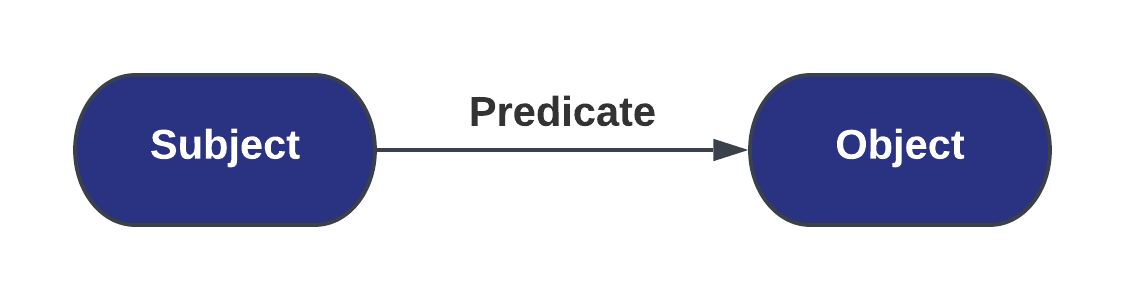
\includegraphics[scale=0.16]{graphics/rdf_triple_simple.png}
        \caption{Example of an RDF triple consisting of a subject, a predicate, and an object.}
        \label{fig:rdf_triple_simple}
    \end{figure}
    
    Figure \ref{fig:rdf_graph_example} shows an RDF graph with two triples in its set. Both triple's subject is the URL of a web page. One triple also has the predicate \textbf{dc:title} and the object \textbf{Building}, whilst the other one has the predicate \textbf{dc:description} and the object \textbf{An ontology of a simple building}. As we can see, each of the RDF terms (subject-predicate-object) can be e.g. URLs or string literals.
    
    
    \begin{figure}[H]
        \centering
        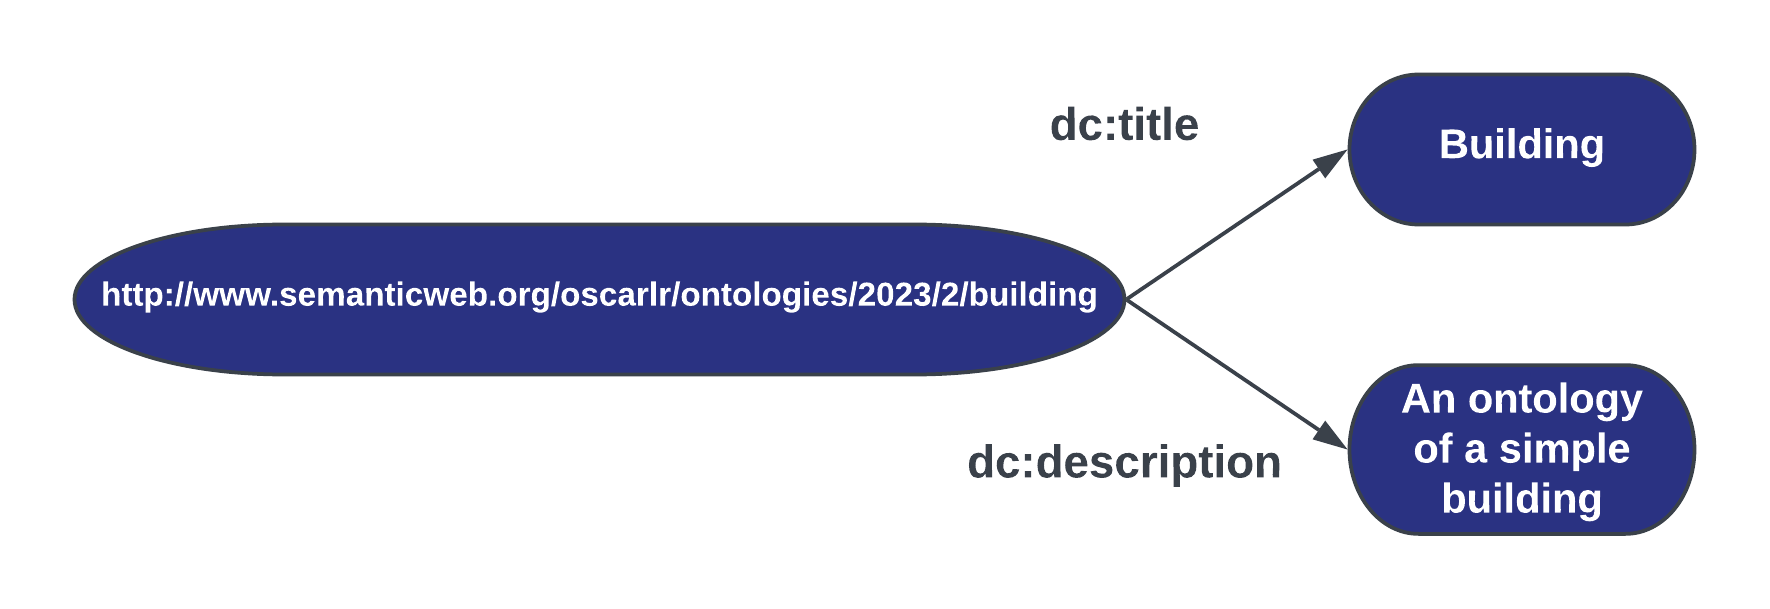
\includegraphics[scale=0.18]{graphics/rdf_graph_example.png}
        \caption{RDF graph consisting of two triples in its set.}
        \label{fig:rdf_graph_example}
    \end{figure}
    \item \textbf{SPARQL}  is a query language for RDF and is defined by W3C. It expresses queries for varying sources of data, and the results from querying are sets of results or RDF graphs \cite{noauthor_sparql_nodate}.
    
    Below is an example of querying the title (\textbf{Building}) in the RDF graph shown in Figure \ref{fig:rdf_graph_example}.
\end{itemize}
\textbf{Data:}
\begin{Verbatim}[breaklines=true,breaksymbol=]
<http://www.semanticweb.org/oscarlr/ontologies/2023/2/building> 
<dc:title> 
”Building”
\end{Verbatim}
\textbf{Query:}
\begin{Verbatim}[breaklines=true,breaksymbol=]
SELECT ?title 
WHERE
{
  <http://www.semanticweb.org/oscarlr/ontologies/2023/2/building> 
  <dc:title> 
  ?title . 
}
\end{Verbatim}
\textbf{Result:}
\begin{table}[H]
    \begin{tabular}{|c|}
        \hline
        \textbf{title} \\
        \hline
        "Building" \\
        \hline
    \end{tabular}
    \caption{Query Result}
    \label{tab:my_label}
\end{table}
    

\begin{itemize}
    \item \textbf{Web Ontology Language (OWL)} is a language for expressing rich knowledge of concepts (phrases in natural language) in an application domain \cite{szolovits_overview_1977}, as well as relations between entities. More specifically, ontologies describe domains in terms of classes, properties, and individuals \cite{bechhofer_owl_2009}.

    \item \textbf{Shapes Constraint Language (SHACL)} is a language for validating an RDF graph against a set of conditions as shapes expressed in another RDF graph. It is said that "data graphs" can be validated against "shapes graphs" \cite{noauthor_shapes_nodate}.
    
    \item \textbf{JSON-LD} JSON-LD is a JSON-based format for encoding and serializing linked data. Although not a well-established standard, it is still defined by W3C.  More specifically, it enables JSON objects to contain \emph{semantic} links \cite{noauthor_json-based_nodate}.
\end{itemize}

Commonly, these technologies can be used to create \emph{semantic} \hyperref[subsec:DigitalTwins]{digital twins}.

\subsection{Asset Model}\label{subsec:AssetModel}
Although BIM (Building Information Modeling) can be used with RDF and JSON to create static building infrastructure as mentioned in \ref{sec:Introduction}(Introduction), some meaning is lost in translation due to a lack of semantic enrichment. BIM can be used in DTs for more context about the built environment which includes asset behavior \cite{godager_concept_2021}. However, a digital twin should aim to have interoperability between heterogeneous data sources.

OWL documents (i.e. ontologies) can easily be created and maintained in ontology editors, such as Protégé\footnote{\url{https://protege.stanford.edu}}. Such a tool can be used to give semantics to e.g. a model of a building, as well as spending less time on creating and maintaining it compared to BIM. 

Figure \ref{fig:building_ontology} shows an example of an ontology of the simple building shown in Figure \ref{fig:simple_building} in Turtle Syntax (i.e. data format for RDF data model \cite{noauthor_terse_nodate}). This ontology uses semantic technologies outlined in Section \ref{subsubsec:Technologies}(Technologies), such as RDF, which again is used by OWL to formalise knowledge in this specific building domain. For a more compact view of the ontology, URLs are removed and the coordinates of the room border corners are purposely left out, and some white space and comments are also removed. We also do not take directions into account meaning the room R1 will always be left of R2, and R2 always to the right of R1. Note that this is just an example of an ontology and that a real building domain would be many times more complex.

According to W3C's documentation, RDF graphs (such as the one shown in aforementioned Figure \ref{fig:building_ontology}) are static snapshots of information, but by giving appropriate vocabulary collections of Internationalized Resource Identifiers (IRIs) \cite{noauthor_rdf_nodate}, observations about entities or groups of entities through time can be captured.

Lastly, this ontology's data can also be reasoned over with technologies outlined in \ref{subsec:Reasoning}(Reasoning), which contains an example of reasoning over an \emph{inconsistent} ontology in Protégé (desktop version of editor), as well as a description on how to make the ontology \emph{consistent}.


\begin{figure}[H]
    \centering
    \caption{Ontology of a simple building with the object properties (hasDoor, hasWallLeft, hasWallRight), the classes (Room, Wall, Door), and the individuals (D, R1, R2, W).}
    \label{fig:building_ontology}
    \begin{Verbatim}[frame=single]
ex:hasDoor rdf:type owl:ObjectProperty .
ex:hasWallLeft rdf:type owl:ObjectProperty .
ex:hasWallRight rdf:type owl:ObjectProperty .

        
ex:Door rdf:type owl:Class .
ex:Room rdf:type owl:Class .
ex:Wall rdf:type owl:Class .

        
ex:D rdf:type owl:NamedIndividual ,
            :Door.
            
ex:R1 rdf:type owl:NamedIndividual ,
            :Room ;
    :hasWallRight :W .
    
ex:R2 rdf:type owl:NamedIndividual ,
            :Room ;
    :hasWallLeft :W .
    
ex:W rdf:type owl:NamedIndividual ,
            :Wall ;
    :hasDoor :D .
    \end{Verbatim}
\end{figure}

\subsection{SMOL}\label{subsec:SMOL}
SMOL is an imperative, object-oriented research language \cite{noauthor_smol_nodate-1}. According to the introduction of the SMOL language, it integrates semantic technologies, and can be used as a framework for creating DTs. For these DTs, the knowledge graphs can be used to capture asset models \cite{noauthor_introduction_nodate}.

The source code of SMOL is publicly available\footnote{\url{https://github.com/smolang/SemanticObjects}}.

\subsubsection{Core Language}\label{subsubsec:CoreLanguage}
The \emph{lexical structure} (i.e. some basic rules for defining how code is written in a given language) of the SMOL language has a grammar that is defined using a simple \emph{EBNF notation} (i.e. notation for formally specifying syntax) as defined by W3C \cite{noauthor_lexical_nodate, noauthor_ebnf_nodate}. What follows is a simple SMOL program that mainly creates a smartphone object and prints \verb|Careful!| if a criterion is met:

\begin{figure}[H]
    \centering
    \caption{A simple SMOL program (file: example.smol)}
    \label{fig:smol_program}
    \begin{Verbatim}[frame=single]
class Smartphone(Int id, String name, Boolean isBlackBerry) end

main
    Boolean isInsideRaspberryField = True;
    Smartphone blackberry = new Smartphone(1, "Evolve", True);

    if (blackberry.isBlackBerry & isInsideRaspberryField) then
        print("Careful!");
    end
end

    \end{Verbatim}
\end{figure}

\subsubsection{SMOL Interpreter}\label{subsubsec:SMOLInterpreter}

The interpreter reads and executes the SMOL program in a given file. The example program (in the file \textbf{example.smol}) shown in Figure \ref{fig:smol_program} was executed in the terminal. Note that the second and fourth line starts with \verb|MO>|. This simply means commands are executed inside the REPL.
\begin{Verbatim}[frame=single]
java -jar smol.jar
MO> reada example.smol
Careful!
MO>
\end{Verbatim}


\subsection{Reasoning}\label{subsec:Reasoning}
OWL was previously mentioned in \ref{subsubsec:Technologies}(Technologies) as a language for expressing rich knowledge of concepts and relations between entities. We should keep in mind, however, that this formalised knowledge should be reasoned over and put in context to draw conclusions based on criteria. There are many technologies that let us do this.
\subsubsection{HermiT}
HermiT is a reasoner for OWL 2 \cite{glimm_hermit_2014}, which is an upgraded version of OWL. \citeauthor{glimm_hermit_2014} describes that the reasoner support both object and data property classification, as well as SPARQL query answering. HermiT is built into the ontology editor Protégé and can be used to reason over an ontology directly in the editor. 

Figure \ref{fig:hermit_in_protege} shows an ontology that is \emph{inconsistent} (an ontology that cannot have any models and entails everything \cite{horridge_explaining_2009, huang_reasoning_2004}). The ontology is inconsistent because the object properties \textbf{hasWallLeft} and \textbf{hasWallRight} are disjoint (having no elements in common), and the individual \textbf{R1} has both object properties. This makes no sense because the room can't have the wall on its left side and at the same time have it on its right side. This could be fixed by simply removing the object property \textbf{hasWallLeft} from the individual according to the context. The effect of an inconsistent ontology is that no meaningful conclusions can be drawn from it \cite{horridge_explaining_2009}.

\begin{figure}[H]
    \centering
    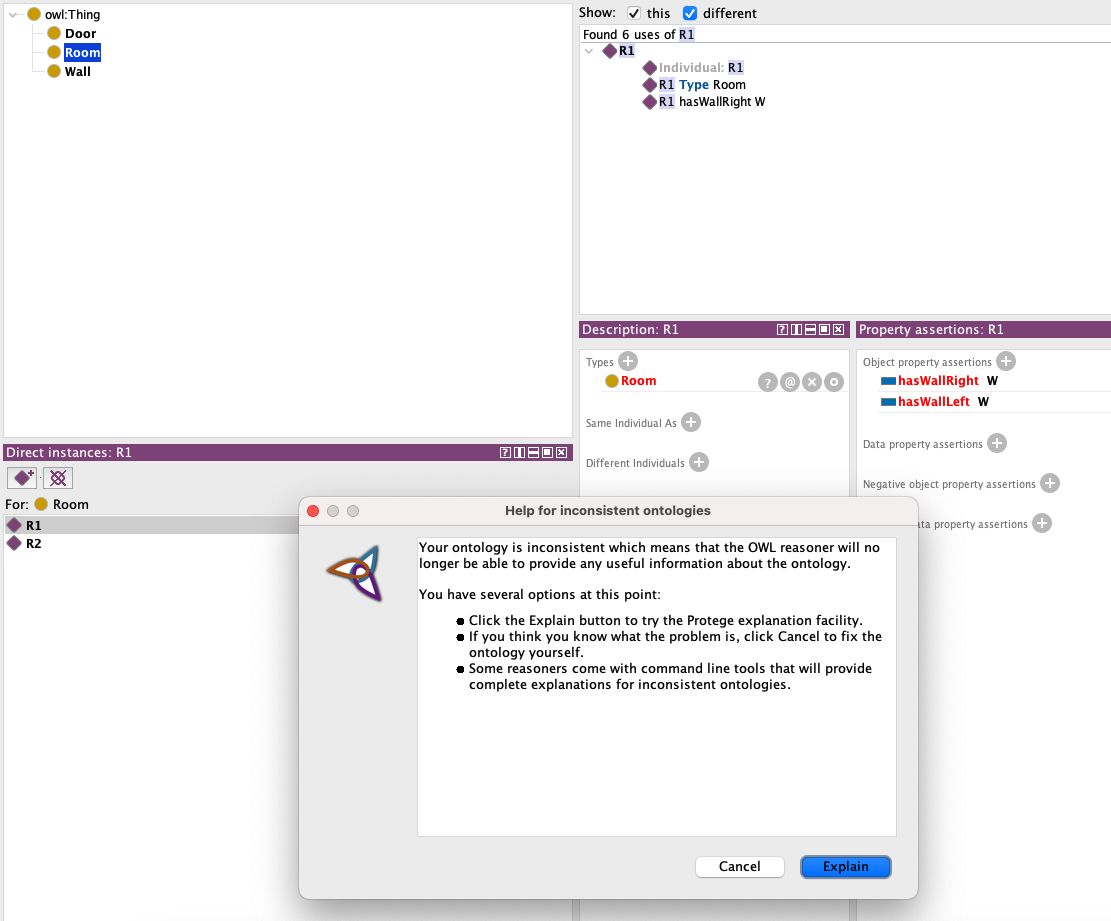
\includegraphics[scale=0.32]{graphics/screenshot_ontology.png}
    \caption{Shows use of HermiT to reason over an ontology directly in Protégé. The information window \textbf{Help for inconsistent ontologies} tells us that the OWL reasoner (HermiT) will no longer be able to provide any useful information about the ontology.}
    \label{fig:hermit_in_protege}
\end{figure}

There also exist other technologies that provide reasoner tools. Some notable mentions include, but are not limited to:
\begin{itemize}
    \item{\textbf{Apache Jena}} is an open source framework that has the Inference API which include reasoner tools that can be used to reason over data, as well as checking content of triple stores \cite{noauthor_apache_nodate-1}. The source code is publicly available\footnote{\url{https://github.com/apache/jena}}.
    \item{\textbf{OWL API}} is a Java framework that lets us create, serialize or manipulate ontologies written in OWL \cite{noauthor_owl_nodate}, and its source code is openly accessible\footnote{\url{https://github.com/owlcs/owlapi}}. Its recent development is more focused towards OWL 2 however.
    \item\hyperref[subsec:SMOL]{\textbf{SMOL}} provide reasoning tools through its interpreter, which implements \emph{semantic lifting} (i.e. generating a knowledge graph from the current state of a SMOL program) \cite{noauthor_semantic_nodate}. 
    
    The knowledge graph is generated by using the \verb|dump| command in SMOLs Read-Eval-Print Loop (REPL) (i.e. user inputs in a terminal are read and results are returned to the user). The knowledge graph is generated as an output file with the filename extension \verb|.ttl|. Reasoning is done automatically by the interpreter whenever \verb|access| or \verb|member| are executed. Apache Jena reasoner is used for \verb|access|, whilst \verb|member| triggers reasoning over an OWL concept with HermiT. Validating with SHAQL does however not require reasoning.
\end{itemize}



\subsection{App Development}\label{subsec:AppDevelopment}
Compared to previously covered topics, such as digital twins (DTs) and the Semantic web, app development is not a well-researched topic, as it is mainly used in industry. We will therefore take an industrial approach in describing the topic of app development.

Smartphones and tablets have different operating systems for mobile, in which the two most notable are iOS (iPhone and iPad) and Android (smartphones and tablets with different brands, such as Samsung, Google, and OnePlus). Smartphones are heterogeneous by nature. They not only have different operating systems but also have various device sensors, depending on the brand and price of the device. 

One should develop for multiple platforms from a single codebase, provided that development time is crucial and that the app should have cross-platform (e.g. both iOS and Android) support. However, this should be planned early on in the development, preferably before anyone starts writing code. Some examples of frameworks that support cross-platform app development include:

\begin{itemize}
    \item Flutter
    \item Ionic
    \item React Native
\end{itemize}

Devices are often equipped with a GPS (Global Positioning System), which gets signals from satellites to determine the GPS-based physical location of the device. Google provides a service, namely Google Location Accuracy, which collects additional location data from multiple sources, such as nearby Wi-Fi and cellular networks, to provide a more accurate physical location of a device \cite{noauthor_how_nodate}. The Google Maps SDK is a set of tools for integrating maps into applications, such as for Android and iOS. According to Google, some features of the Software Development Kit (SDK) are different map displays and map gesture responses \cite{noauthor_maps_nodate}.

\subsection{Databases}\label{subsec:Databases}
Databases are collections of information that exist for a long time, often over many years \cite{garcia-molina_database_2002}. They can be divided into relational and non-relational (NoSQL) databases and are often compared as such \cite{mohamed_relational_2014}. Relational databases have existed for many decades and store data in tables (which consist of columns and rows), whilst \emph{NoSQL} (i.e. not only SQL) databases store data in JSON documents \cite{garcia-molina_database_2002, sudiartha_data_2020}. Examples of relational databases are MySQL and PostgreSQL, whereas examples of NoSQL databases are: 
\begin{itemize}
    \item \textbf{MongoDB} is a well-known NoSQL database for storing data in JSON documents and its source code is publicly available\footnote{\url{https://github.com/mongodb/mongo}}.
    \item \textbf{Firebase Realtime Database} is a cloud-hosted NoSQL database that stores data as JSON objects  \cite{noauthor_firebase_nodate}. Furthermore, data is synchronized in real-time to cross-platform clients.
    \item \textbf{InfluxDB} is a NoSQL database for storing \emph{time series data} (i.e. "sequence of data points indexed in time order" \cite{noauthor_what_nodate})  \cite{noauthor_influxdb_nodate}, and its source code is also openly accessible\footnote{\url{https://github.com/influxdata/influxdb}}.
\end{itemize}

According to \citeauthor{garcia-molina_database_2002}, databases are managed by a Database Management System (DBMS), a system that should:
\begin{itemize}
    \item Let users create new databases in which the logical structure of data (schema) is specified by the user using a data-definition language.
    \item Let users query and modify data with a query language.
\end{itemize}

Non-relational variants have become increasingly popular in recent years due to how they solve scalability concerns with relational databases. NoSQL databases are of different types, such as document databases and graph databases. As described by \citeauthor{mohamed_relational_2014}, traditional databases were not created with horizontal scaling (sharding) in mind. More specifically, it does not do well with new machines being added to the pool of resources. Instead, it relies heavily on vertical scaling, which is adding more computing power (CPU, RAM) to an individual resource (machine) in the pool. On the other hand, NoSQL databases are optimized for scaling horizontally \cite{mohamed_relational_2014, kim_geoycsb_2023}.

We should consider that although databases can have many different uses, some are better for specific purposes than others. Time series databases can be integrated into digital twins (DTs) for getting updated sensor data from the physical twin (PTs). \ref{subsec:SMOL}(SMOL) describes that SMOL can be used as a framework to create DTs. Additionally, in SMOL we can query time series data from InfluxDB by using the \verb|access| statement \cite{noauthor_time_nodate}. An example program of querying latitude and longitude coordinates from the start of the time range, and then returning the list of coordinates follows:

\begin{figure}
    \centering
    \begin{Verbatim}[frame=single,breaklines=true]
List<Double> getCoordinates()
    List<Double> coordinates = null;
    coordinates = access(
        "from(bucket: \"Data\")
        |> range(start: 0)
        |> filter(fn: (r) => r[\"_measurement\"] == \"data\")
        |> filter(fn: (r) => r[\"_field\"] == \"latitude\" or r[\"_field\"] == \"longitude\")
        |> aggregateWindow(every: 5m, fn: mean, createEmpty: false)
        |> yield(name: \"mean\")",
        INFLUXDB("influx.yml")
    );
    return coordinates;
end
    \end{Verbatim}
    \caption{Accessing time-series data from InfluxDB in a function written in SMOL.}
    \label{fig:access_time_series}
\end{figure}
    

Firebase Realtime Database has multi-platform support for clients, such as support for Android and iOS devices \cite{noauthor_firebase_nodate}.



\newpage
\section{Problem analysis and design}\label{sec:Analysis}
This chapter examines the problem statement (H) and its three guiding research questions (RQ1, RQ2, RQ3) in \ref{sec:Introduction}(Introduction), based on the theoretical background information and general code examples in \ref{sec:Background}(Background). We create a building domain based on the analysis of the research questions. Then we examine what a dynamic asset model entails, and how static data can be separated from dynamic data in it. Different technologies described in \ref{sec:Background}, such as databases, frameworks for creating applications (apps), and semantic digital twins are considered. Lastly, we present the resulting structural requirements as the basis for the implementation.

\subsection{Research questions}
To better understand what we should analyze, we should take an extra look at the hypothesis (H), as well as the three research questions (RQ1, RQ2, RQ3). We also look at how they adhere to the problem statement.

\begin{itemize}
    \item[\textbf{H:}] We can handle mobile assets in a semantic digital twin with the use of a dynamic asset model of a simple building, in which dynamic data (smartphone's physical location) is automatically updated by a server and separated from static data (existing building infrastructure), and informed decisions are sent back to the physical twin.
    \item[\textbf{RQ1:}]
    Can we create a dynamic asset model of a simple building that is also extensible?
    \item [\textbf{RQ2:}] 
    Can we enable bidirectional data flow between the PT and DT, such that the digital twin gets updated sensor data from mobile devices and sends informed decisions back?
    \item [\textbf{RQ3:}]
    Can we clearly separate dynamic data (smartphone's position) from static data (building infrastructure) in the asset model and in the DT?
\end{itemize} 

\subsubsection{First research question (RQ1)}
RQ1 asks if we can "create a dynamic asset model of a simple building that is also extensible". An asset model (ontology) is simply an OWL document (file) that is exported from creating an ontology in an ontology editor, such as Protégé. Although other ontology editors can be used, we should use Protégé due to its user-friendliness and the extensive documentation provided in the user guide \cite{horridge_practical_2011}. This exported file is provided to and used by the digital twin (DT) by using the SMOL interpreter. The section below in \ref{subsubsec:DynamicAssetModel}(Dynamic Asset Model) examines what a \emph{dynamic} asset model entails. 

The 1st research question also focuses on creating an asset model of a simple building that is \emph{extensible}. To add to this, being extensible means that an operator should be able to manually add new smartphones that have no registered physical location yet or add existing building infrastructure to the ontology. It should be possible to manually edit the static parts of the asset model if the building domain changes (e.g. a door is added to a wall) as well. 

A digital twin (DT) based on a \emph{dynamic} asset model should be able to recognize the following, according to the generated knowledge graph:
\begin{itemize}
    \item Manual changes of static data by an operator
    \item Automatic updates of dynamic positional data from the server
\end{itemize}

\subsubsection{Second research question (RQ2)}\label{subsubsec:RQ2}
RQ2 asks whether we can "enable bidirectional data flow between the PT and DT, such that the digital twin gets updated sensor data from the mobile devices in the PT and sends informed decisions back". Bidirectional data flow is data that is exchanged both ways, and not just in one direction between the physical twin (PT) and digital twin (DT), or vice versa. The DT observes the PT in near real-time and gets updated sensor data from its physical counterpart. The DT should then send informed decisions back to it. A lot of value is derived from the DT making an informed decision on behalf of a mobile asset in the PT, and it is crucial that the appropriate smartphone user is notified.

The DT could conclude to make an informed decision if some criteria are met. As an example of a criteria, we look at how we can check if a smartphone is inside a critical area. Using what is shown in Figure \ref{fig:simple_building} as a basis, an area's two border corners are expressed as follows:
\begin{enumerate}
    \item $(x_1, y_1)$
    \item $(x_2, y_2)$
\end{enumerate}
Meaning, if we want to check if a smartphone's physical location (point) $(x, y)$ is inside such an area, we can check if the following is true:\newline\newline$(x >= x_1\:AND\: x <= x_2)\:OR\:(x >= x_2\:AND\:x <= x_1)$\newline$AND$\newline$(y >= y_1\:AND\:y <= y_2)\:OR\:(y >= y_2\:AND\:y <= y_1)$\include\newline We also include both directions so maintainers can freely choose border corners for an area, which makes it easier to use and aligns with the RQ1.


\subsubsection{Third research question (RQ3)}
RQ3 is concerned with if we can "clearly separate dynamic data (smartphone's position) from static data (building infrastructure) in the asset model and in the DT". The hypothesis (H) states that the asset model should be of a simple building, which means some data don't have to change as existing building infrastructure can be expressed with \emph{static data} based on coordinates of the room border corners as shown in Figure \ref{fig:simple_building}. The room(s) as square area(s) constitute a simple building. In contrast to static data, the mobile assets can change at any time, and their physical location also changes constantly hence their positional data is \emph{dynamic}.

\subsection{Building domain}
From considering the three research questions, we have created a possible domain including a built environment based on static data, as well as movable entities with their physical location as dynamic data, as shown in Figure \ref{fig:static_built_environment}. \textbf{Physical 2D space} is provided for context of outside and is in two dimensions as described in \ref{subsec:Scope}(Thesis scope and outline). This means that altitude is not taken into account. Note that the relationships between some entities use \emph{composition} (i.e. indicates a very strong relationship between the entities, which means that if the owing entity (e.g. \textbf{Physical 2D space}) is destroyed, so is the entity linked to it (e.g. \textbf{Building} \cite{pilone_uml_2005}) (it can be thought of as a black hole..)

\begin{figure}[H]
    \centering
    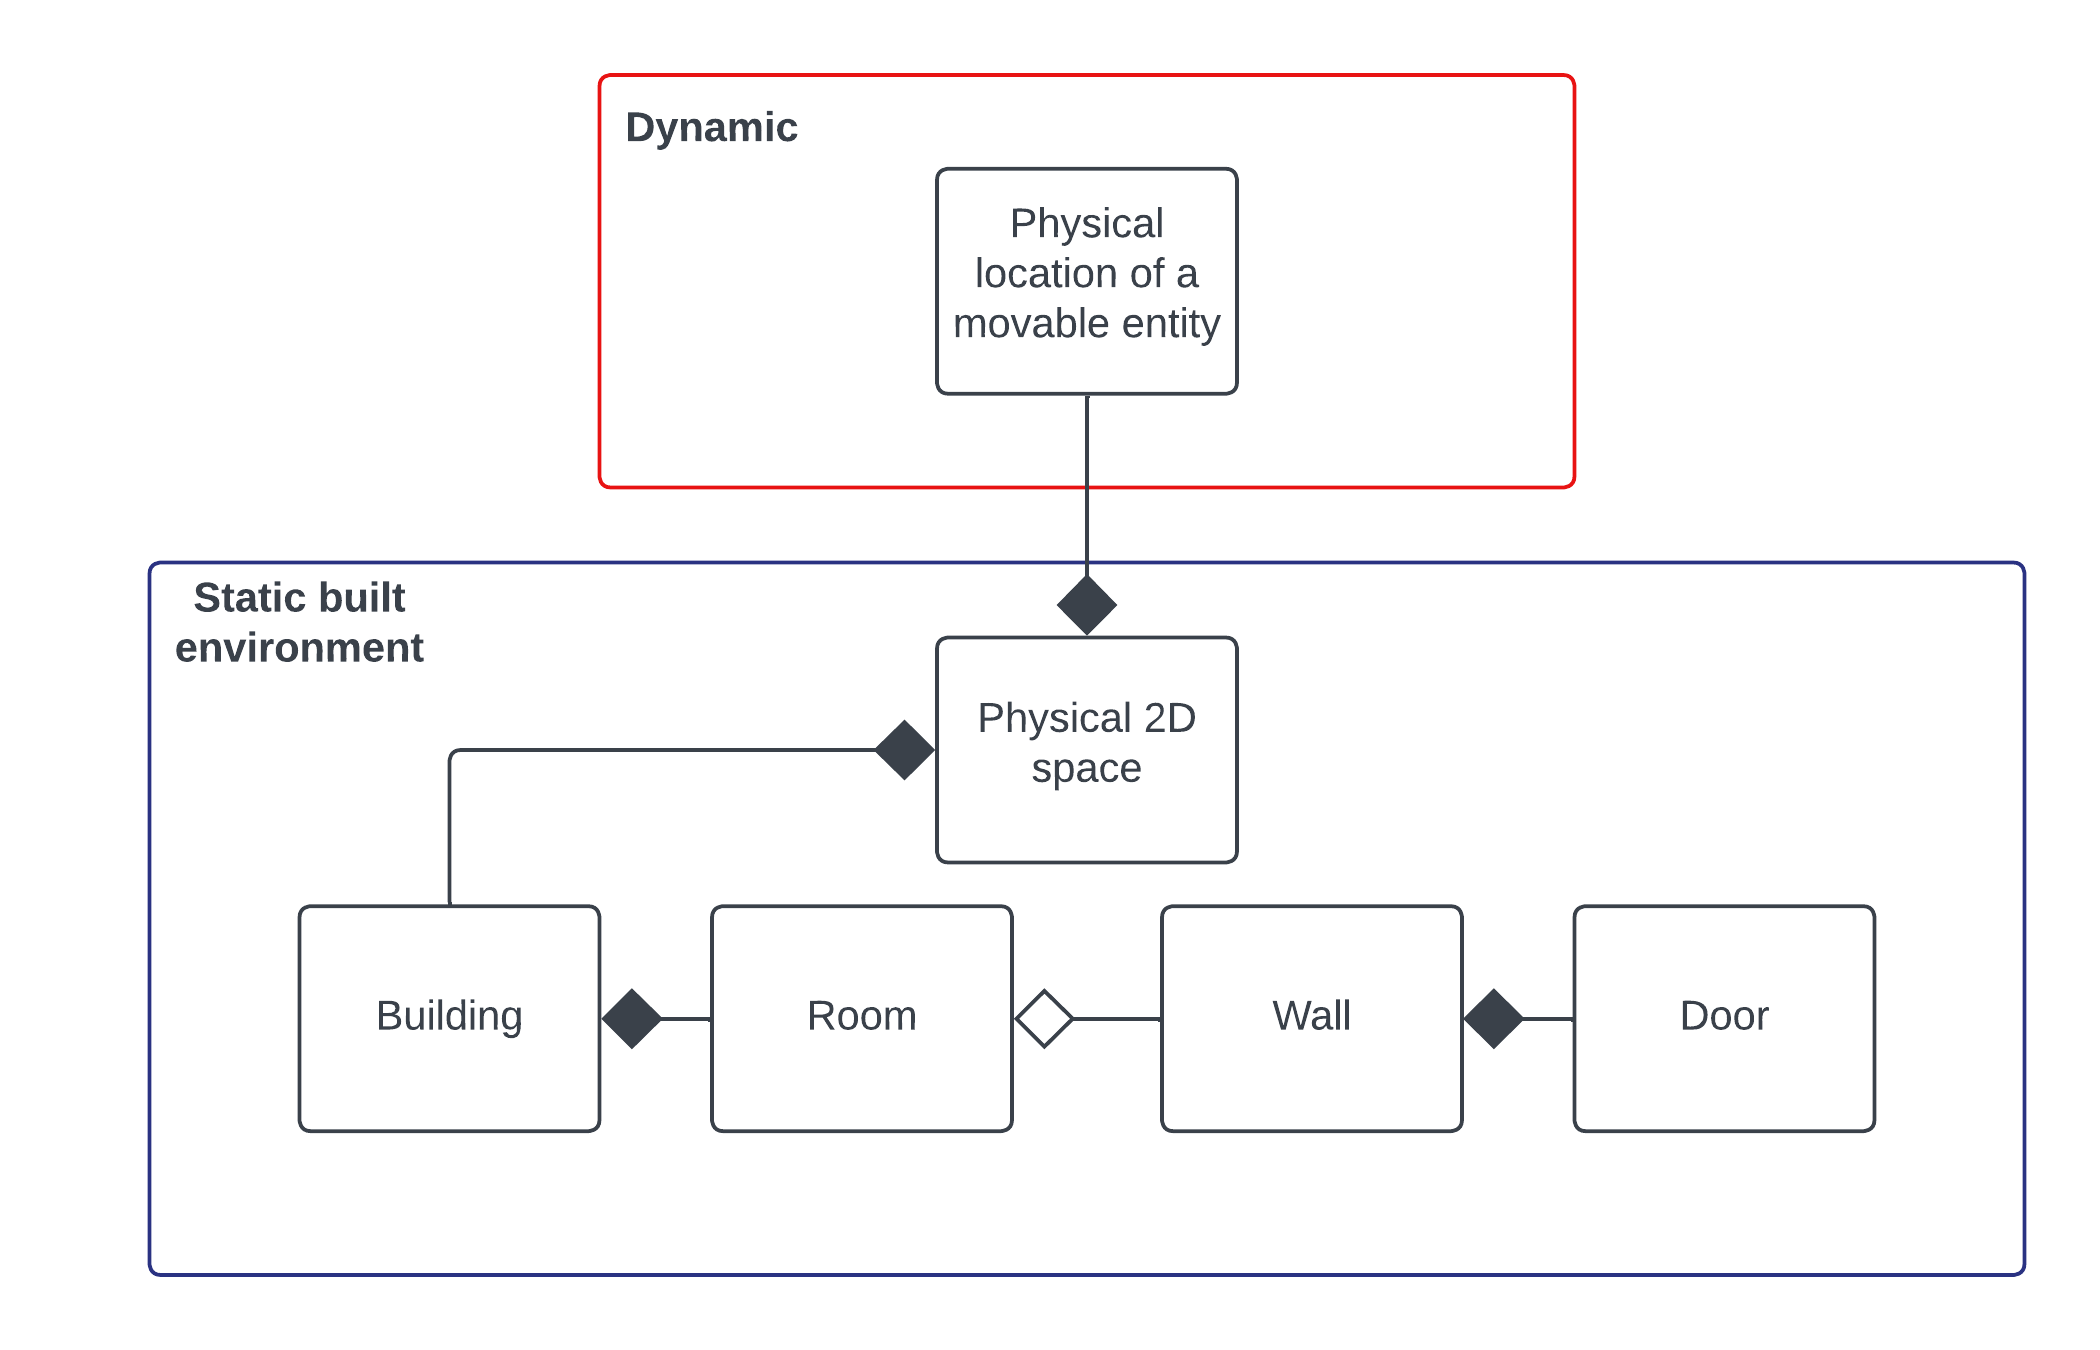
\includegraphics[scale=0.16]{graphics/static_built_environment.png}
    \caption{A UML class diagram that illustrates the separation of static and dynamic behavior.}
    \label{fig:static_built_environment}
\end{figure}


\subsection{Dynamic asset model}\label{subsubsec:DynamicAssetModel}
Section \ref{subsec:AssetModel}(Asset Model) describes concerns with BIM (Building Information Modeling), and how ontologies (asset models) created with semantic technologies deal with these concerns. Another concern with BIM worth mentioning is that it does not handle dynamic behavior very well \cite{kamburjan_digital_2022}.

Simply put, a \emph{dynamic} asset model is an ontology in which some data changes through time. If we were to export the ontology created in Protégé, we would get an OWL document (file) that would describe the domain in terms of classes, properties, and individuals. Changing the ontology in any way (e.g. adding another movable entity) would represent a new RDF (Resource Description Framework) graph.

Figure \ref{fig:building_ontology} shows an exported ontology of a building in Turtle Syntax. The ontology editor lets us specify the format of the ontology to be exported. From creating this ontology as a basis for our future ontology implementation, we discovered that it would be necessary to create a common class for \emph{atleast} the movable entities (individuals) due to the sheer number of them in the GUI (Graphical User Interface) in Protégé, as well as to formalize the knowledge of heterogeneous smartphones.

\subsection{Data separation}
In this section, we are further analyzing the separation of static and dynamic data and giving some practical examples with text color to support this. First, we describe and illustrate how they can be separated in the asset model and in SMOL. Then we examine how we can separate the static analysis of what a critical area \emph{is} from the dynamic snapshots of smartphones at a certain point in time.

\subsubsection{Static and dynamic data}\label{subsubsec:StaticAndDynamicData}
Figure \ref{fig:static_dynamic_asset_model} shows the separation of static and dynamic data. The \textbf{Asset Model} \emph{doesn't} have dynamic positional data, but the smartphone individuals and their IDs as static data. The SMOL program accesses the smartphones by their IDs with \verb|access|, and adds the positional data from InfluxDB according to the ID. \textbf{Place} consist of area(s) with predefined border corner coordinates and is static data. We take notice that a server could continuously update the time series database with the physical locations of the mobile devices, as well as add the smartphone individuals to the asset model.

The aforementioned figure also shows the direction of data flow between the \textbf{Asset Model} and \textbf{SMOL}, and \textbf{InfluxDB} and \textbf{SMOL}. The SMOL program accesses the static data (\textbf{Place} and instances of \textbf{Smartphone}) in the asset model and gets the updated positional data of the smartphones from InfluxDB. The SMOL program then creates \textbf{Smartphone} objects from the data. The knowledge graph can then be generated and will reflect the separation of static and dynamic data from a combination of the program state and the knowledge base.

\begin{figure}[H]
    \centering
    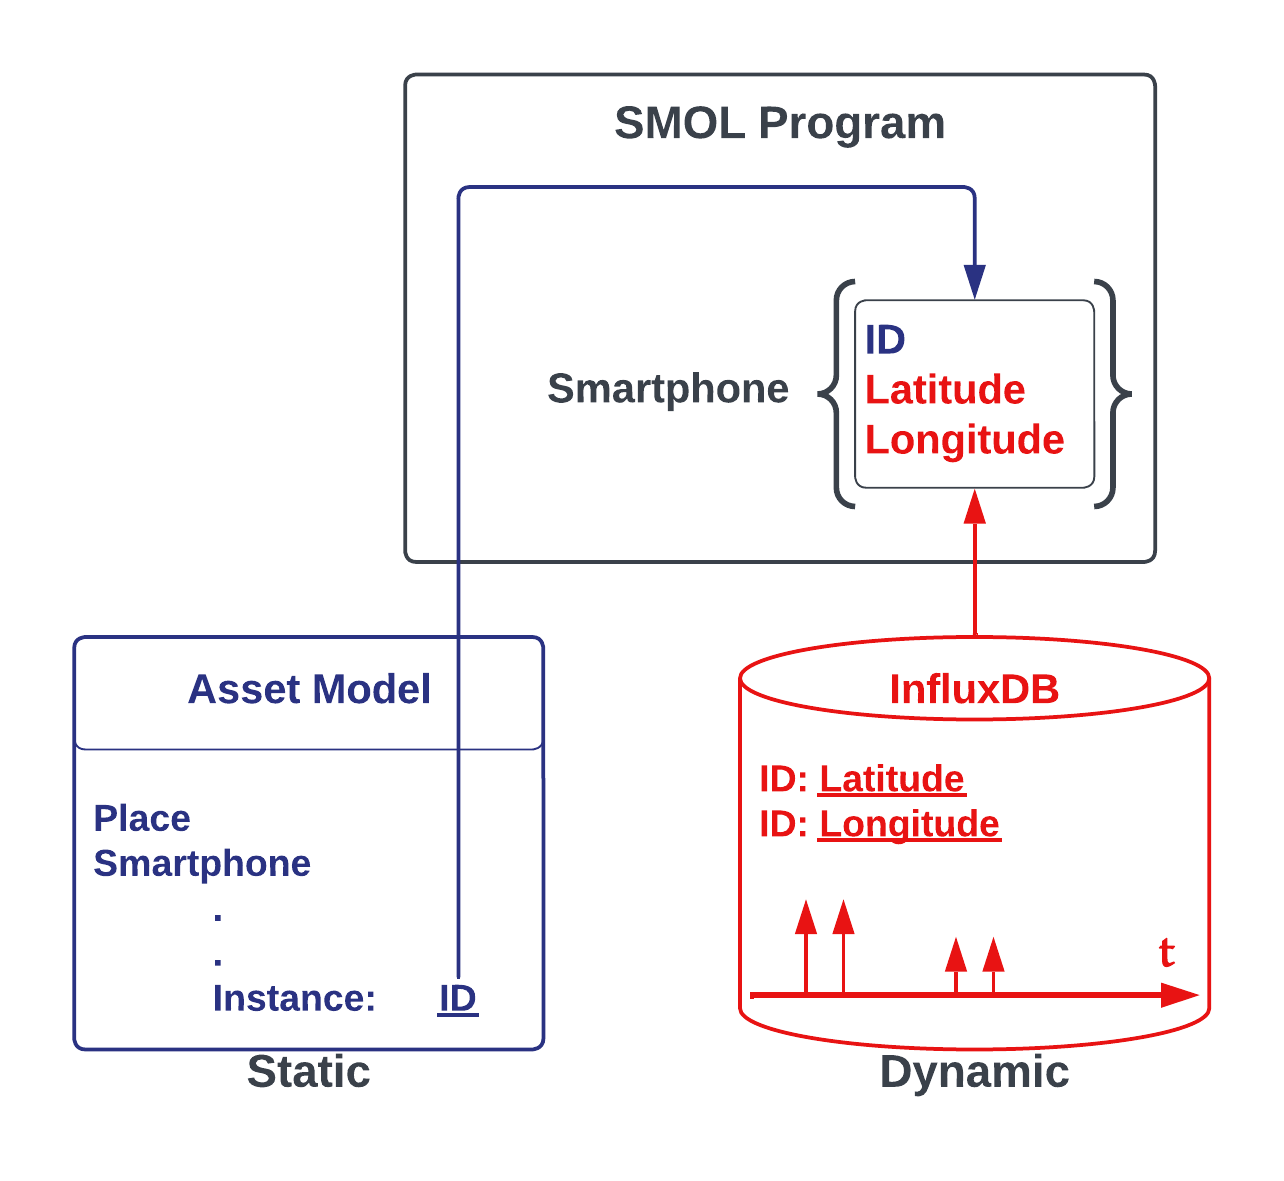
\includegraphics[scale=0.24]{graphics/static_dynamic_asset_model.png}
    \caption{The separation of static and dynamic data. Static data is illustrated in blue, whilst dynamic data is illustrated in red.}
    \label{fig:static_dynamic_asset_model}
\end{figure}

Research question 1 (RQ1) is concerned with an asset model that is \emph{extensible}. Since the smartphone individuals are added to the asset model without positional data, they can also serve as a template for registering new smartphones in the domain. To do this, one can simply add the following to the OWL document (file), where only the numbers highlighted in yellow need to be changed:

\begin{Verbatim}[commandchars=\\\{\}, breakanywhere=true]
### http://www.semanticweb.org/oscarlr/ontologies/2023/2/building#smartphone\hl{5}
:smartphone\hl{5} rdf:type owl:NamedIndividual ,
                      :MovableEntity ;
             :movableEntityId "\hl{5}" .
\end{Verbatim}

\subsubsection{Further data separation}\label{subsubsec:FurtherDataSeparation}
If we were to illustrate querying an asset model with a SPARQL query (SPARQL Query Language for RDF), the consensus is to use red color for core parts of SPARQL syntax or language, whilst the color blue is used for examples of query-specific values or text that goes into SPARQL queries \cite{noauthor_sparql_nodate}. Keeping this in mind, we still use blue text color for static data and red text color for dynamic data in this thesis because they are, respectively, calming or disruptive. 

It is important to look at the differences between the sensor data and the informed decisions in terms of what the data can be used for. The DT gets updated sensor data from the PT, and sends informed decisions back, as RQ2 states. The updated sensor data from the PT is the newest physical location from the mobile assets in the PT. It is crucial that the PT can use this data \emph{as is}, and therefore the data should be exact coordinates (latitude, longitude), and identifiable. We should think about what an informed decision means. An informed decision is a conclusion made by the DT when there is sufficient information to determine something on behalf of the PT to control it. An example of this is the DT sending warnings back to the PT when the DT has determined that smartphones are inside critical areas. The analysis of what a critical area \emph{is} however, is not taken into account, as stated in \ref{subsec:Scope}(Thesis scope and outline). Therefore, the DT should not decide that an area is dangerous. This could be a job for an operator responsible for defining the areas in the asset model. 

Lastly, we should separate the static analysis of what a critical area is from the dynamic snapshots of smartphones at a certain point in time. This way the dynamic behavior doesn't affect the static behavior. Some background information on a digital shadow (DS) was given in \ref{subsec:DigitalTwins}(Digital Twins). A DS could be created to handle one-way data flow and to further separate data, as well as give modularity to our implementation.

\subsection{Analysis of technologies}
In this section, we analyze different technologies, such as \ref{subsec:AppDevelopment}(App Development), \ref{subsec:Databases}(Databases), and \ref{subsec:DigitalTwins}(Digital Twins) from the descriptions of them in \ref{sec:Background}. These technologies can be used to realize the proposed high-level architecture in Figure \ref{fig:initial_components}. Choices of architectural components are justified based on the analysis of the problem space. We look at time series databases and real-time databases, frameworks for creating cross-platform apps, and semantic digital twins.

\subsubsection{App Development}\label{subsubsection:AppDevelopment}
From the background information on application development provided in \ref{subsec:AppDevelopment}(App Development), we chose to focus on Flutter as a framework for creating cross-platform applications (apps) due to a number of reasons. We considered other frameworks for creating apps for iOS and Android from a single codebase as well, such as Ionic and React Native. However, we had no prior experience with either, and Flutter has great documentation provided by Google, and is praised by developers at Stack Overflow (an online community for developers) \cite{noauthor_why_nodate}.

The programming languages were seen as tools that came with the choice of frameworks and were thus not focused on that much. However, the programming language used in Flutter applications is Dart, which is also developed by Google. React Native and Ionic apps are both written in JavaScript. Ionic apps can be written using a single code base in the libraries React, Angular, or Vue \cite{noauthor_ionic_nodate}.

\subsubsection{Databases}\label{subsubsection:Databases}
There exist many databases, but the section \ref{subsec:Databases}(Databases) narrowed the possible choices down to the time series database InfluxDB and the real-time database provided by Firebase. 

SMOL, as a framework for creating digital twins (DTs), supports InfluxDB and provides open-source examples for querying time series data which made it an easy choice. 

When it comes to real-time databases, we saw that the real-time database by Firebase is based on web-sockets, which is more performant than polling due to data being accessed in real-time and due to low latency. There is also no limit to the number of nodes that can be pushed to a list in Firebase, which let us handle an unlimited number of smartphones as stated in \ref{subsec:Scope}. Although this can be very costly if the user base scales out of proportion. Redis was also considered as a real-time database that could be used for our implementation, but we had prior experience with Firebase, and integrating it should take less time. It is a cloud-hosted solution \cite{noauthor_firebase_nodate} and one can download the Google Cloud SDK Shell to authenticate and interact with the services provided by Firebase.

Furthermore, using a database in the communication between clients and the server allows for an operator to easily check the assigned clients, as well as which clients should be informed. From our early implementation, it was made clear that \emph{real physical devices} (not just emulated ones) should be detected by the physical twin (PT). 

Lastly, we should ask ourselves why we should use a real-time database in our client-server communication, but this is later discussed in \ref{subsec:ClientServerCommunication}(Client-server communication) where we also look at FastAPI and communication between architectural components.

The \textbf{Server} in Figure \ref{fig:initial_components} has not been explicitly described yet in this thesis as its main function was to enable a bidirectional flow of data between the PT and the digital twin (DT). Most people in general are familiar with Java,  a well-known and established programming language, and our fellow students are quite familiar with its syntax as well. Lastly, The OWL API and Apache Jena have many open-source examples in Java, which is another reason we should use Java in our server implementation and not e.g. Kotlin (which the SMOL interpreter is written in). 

\subsubsection{Semantic Digital Twins}\label{subsubsec:SemanticDigitalTwins}
\ref{subsec:SMOL}(SMOL) describes that SMOL (Semantic Micro Object Language) can be used as a framework for creating digital twins (DTs) and that it integrates semantic technologies. Knowledge graphs can be generated by using the \verb|dump|-command in the REPL provided by the SMOL interpreter. The knowledge graph can capture a knowledge base, such as a dynamic asset model, in which static data is separated from dynamic data. This asset model combined with the SMOL program, produces the knowledge graph. It is also possible to access the asset model from the SMOL program. As SMOL also integrates semantic languages, such as SHACL for validation and SPARQL for querying, it could be a good fit for our implementation.

\subsection{Structural requirements}\label{subsec:Requirements}
We have analyzed the research questions, the building domain, and the dynamic asset model in which static and dynamic data are separated. Technologies have also been examined and justified. From this, we create the structural requirements for the implementation, which is an \emph{unordered} nested list in which all levels are also \emph{unordered}. It is structured into the parts \textbf{Client}, \textbf{Server}, \textbf{Databases}, and \textbf{Digital Twin}.
\newline

\noindent\textbf{Structural requirements:}
\begin{itemize}
    \item \textbf{Client}
    \begin{itemize}
        \item Client can choose to send its newest status (ID, latitude, longitude) 
        \item Appropriate endangered clients need to be warned 
        \item Show appropriate in-app messages to the user
        \item Ask for permission to track the physical position of the device
        \item Clearly show when the physical location of the device is tracked
        \item Clearly show when the physical location of the device is \emph{not} tracked
    \end{itemize}
    \item \textbf{Server}
    \begin{itemize}
        \item \textbf{1.} Forward the sensor data to a time series database, which the DT accesses
        \item \textbf{2.} Forward the informed decisions to a real-time database, which the PT accesses
        \item Should be possible to do \textbf{1.} and \textbf{2.} above at the same time
        \item Reloads asset model with tracked clients
        \item Access and read the generated knowledge graph
    \end{itemize}
    \item \textbf{Databases}
    \begin{itemize}
        \item Realtime database
        \begin{itemize}
            \item Store the ID and physical location of the clients
            \item Store data about which clients (in the PT) the DT made an informed decision on behalf of
        \end{itemize}
        \item Time series database
        \begin{itemize}
            \item Store the time series data
        \end{itemize}
    \end{itemize}
    \item \textbf{Semantic Digital Twin}
    \begin{itemize} 
        \item \textbf{3.} DS gets the newest sensor data from the time series database
        \item \textbf{4.} Access the smartphones by their IDs in the asset model
        \item Create smartphone objects by combining data from \textbf{3.} and \textbf{4.} above. 
        \item Access \emph{only} the areas from the asset model that are \emph{critical}
        \item Check if smartphones are inside any critical areas
        \item Handle if there are any smartphones that don't have a registered physical location
        \item Provide examples of SPARQL queries
        \item Show informative messages in the REPL during program execution
    \end{itemize}
\end{itemize}

In addition to this, operators should be able to access the knowledge graph and edit the asset model either offline or online. Lastly, it should be possible for an administrator to check the data stored in both the real-time database and the time-series database, whilst protecting clients' privacy as much as possible.

\newpage


\section{Implementation}\label{sec:Implementation}
This chapter describes the proof-of-concept implementation based on the structural requirements in \ref{subsec:Requirements}(Structural requirements), by describing each of the following parts in it:
\begin{itemize}
    \item Client
    \item Server
    \item Databases
    \item Semantic Digital Twin
\end{itemize}
In the first section we describe an \emph{early version} of the final implementation based on the initial architecture of software components in Figure \ref{fig:initial_components}. 

Then we look at the revised final version in Figure \ref{fig:components}, and describe what we implemented. For each of the larger architectural components in the figure, we reference the section that describes it in \ref{sec:Background}(Background), and the design decision that enables it in \ref{sec:Analysis}(Analysis and design). We also reference the corresponding \emph{item} in the structural requirement \emph{part} we are in.

\subsection{Early implementation}\label{subsec:EarlyImplementation}
Due to the extensive architecture, we chose to implement an early version by letting all of the architectural components in Figure \ref{fig:initial_components} communicate first. The \textbf{Physical Twin} in the figure consists of \textbf{Mobile Assets} which are smartphones. Based on the background information in \ref{subsec:AppDevelopment}(Background - App Development), and from further narrowing of the technologies in \ref{subsubsection:AppDevelopment}(Analysis - App Development), a Flutter app was created for cross-platform support.

Figure \ref{fig:recording_off} and \ref{fig:recording_on} show the location recording toggle function in the app, off and on, respectively. The recording is off by default, and when the button is pressed, it starts tracking the position of the device and changes color. Then when it is pressed again, the latest physical location of the device is sent, alongside its ID, as a status message to the server over TCP (Transmission Control Protocol).

\begin{figure}[H]
    \centering
    \begin{minipage}[c]{0.34\linewidth}
        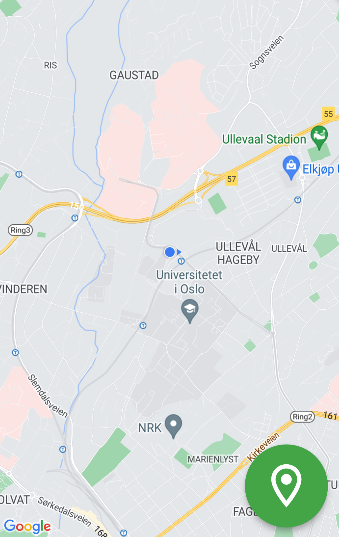
\includegraphics[width=\linewidth]{graphics/recording_off.png}
        \caption{Shows that the location recording is off (green button).}
        \label{fig:recording_off}
    \end{minipage}
    \hfill
    \begin{minipage}[c]{0.34\linewidth}
        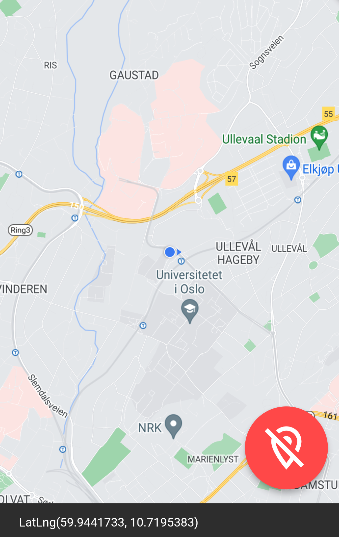
\includegraphics[width=\linewidth]{graphics/recording_on.png}
        \caption{Shows that the location recording is on (red button).}
        \label{fig:recording_on}
    \end{minipage}
\end{figure}

We created a Maven project (a tool for managing the project) and used the object-oriented programming language Java for the server implementation. To let the server track many clients, we first assigned an ID to the client when it connected to the server, and kept track of all assigned clients. The client received its assigned ID from the server which was later sent alongside the client's physical location as status update messages when pressing the button again. As this was an early implementation, we implemented client-server communication over TCP (Transmission Control Protocol) which is further discussed in \ref{subsec:ClientServerCommunication}(Client-server communication).

An asset model (ontology) of a simple building was also created as shown in Figure \ref{fig:simple_building} (this time with coordinates as data properties which were "added" to individuals of the \verb|MovableEntity| class suggested in \ref{subsubsec:DynamicAssetModel}(Dynamic asset model). We used Protégé to create the domain and exported it as an OWL document (file). This file was then accessed in a new SMOL program based on the background information in \ref{subsubsec:Technologies}(Technologies) and \ref{subsubsec:CoreLanguage}, and from further analysis in \ref{subsubsec:StaticAndDynamicData}(Static and dynamic data). 

To sum up, in the early version of the implementation a simple app was created to send sensor data (physical location from GPS-sensor in the devices as described in \ref{subsec:AppDevelopment}) to a server. Furthermore, the file containing information about a simple building domain was accessed in SMOL.


\subsection{Implemented solution}\label{subsec:ImplementedSolution}
Figure \ref{fig:components} shows the architectural components in the final implementation. More specifically, it illustrates the \textbf{Mobile Assets} in the \textbf{Physical Twin}, its \textbf{Digital Twin} based on a dynamic \textbf{Asset Model}, and the \textbf{Server} which enables the communication between the PT and DT both ways. In addition to this, the figure illustrates that \textbf{Firebase Realtime database} is used as a channel between the \textbf{Physical Twin} and the \textbf{Server}, and that \textbf{InfluxDB time-series database} is used for storing the sensor data which \emph{can} be accessed from the \textbf{SMOL} program, as shown in the example function in \ref{fig:access_time_series}.

\begin{figure}[H]
    \centering
    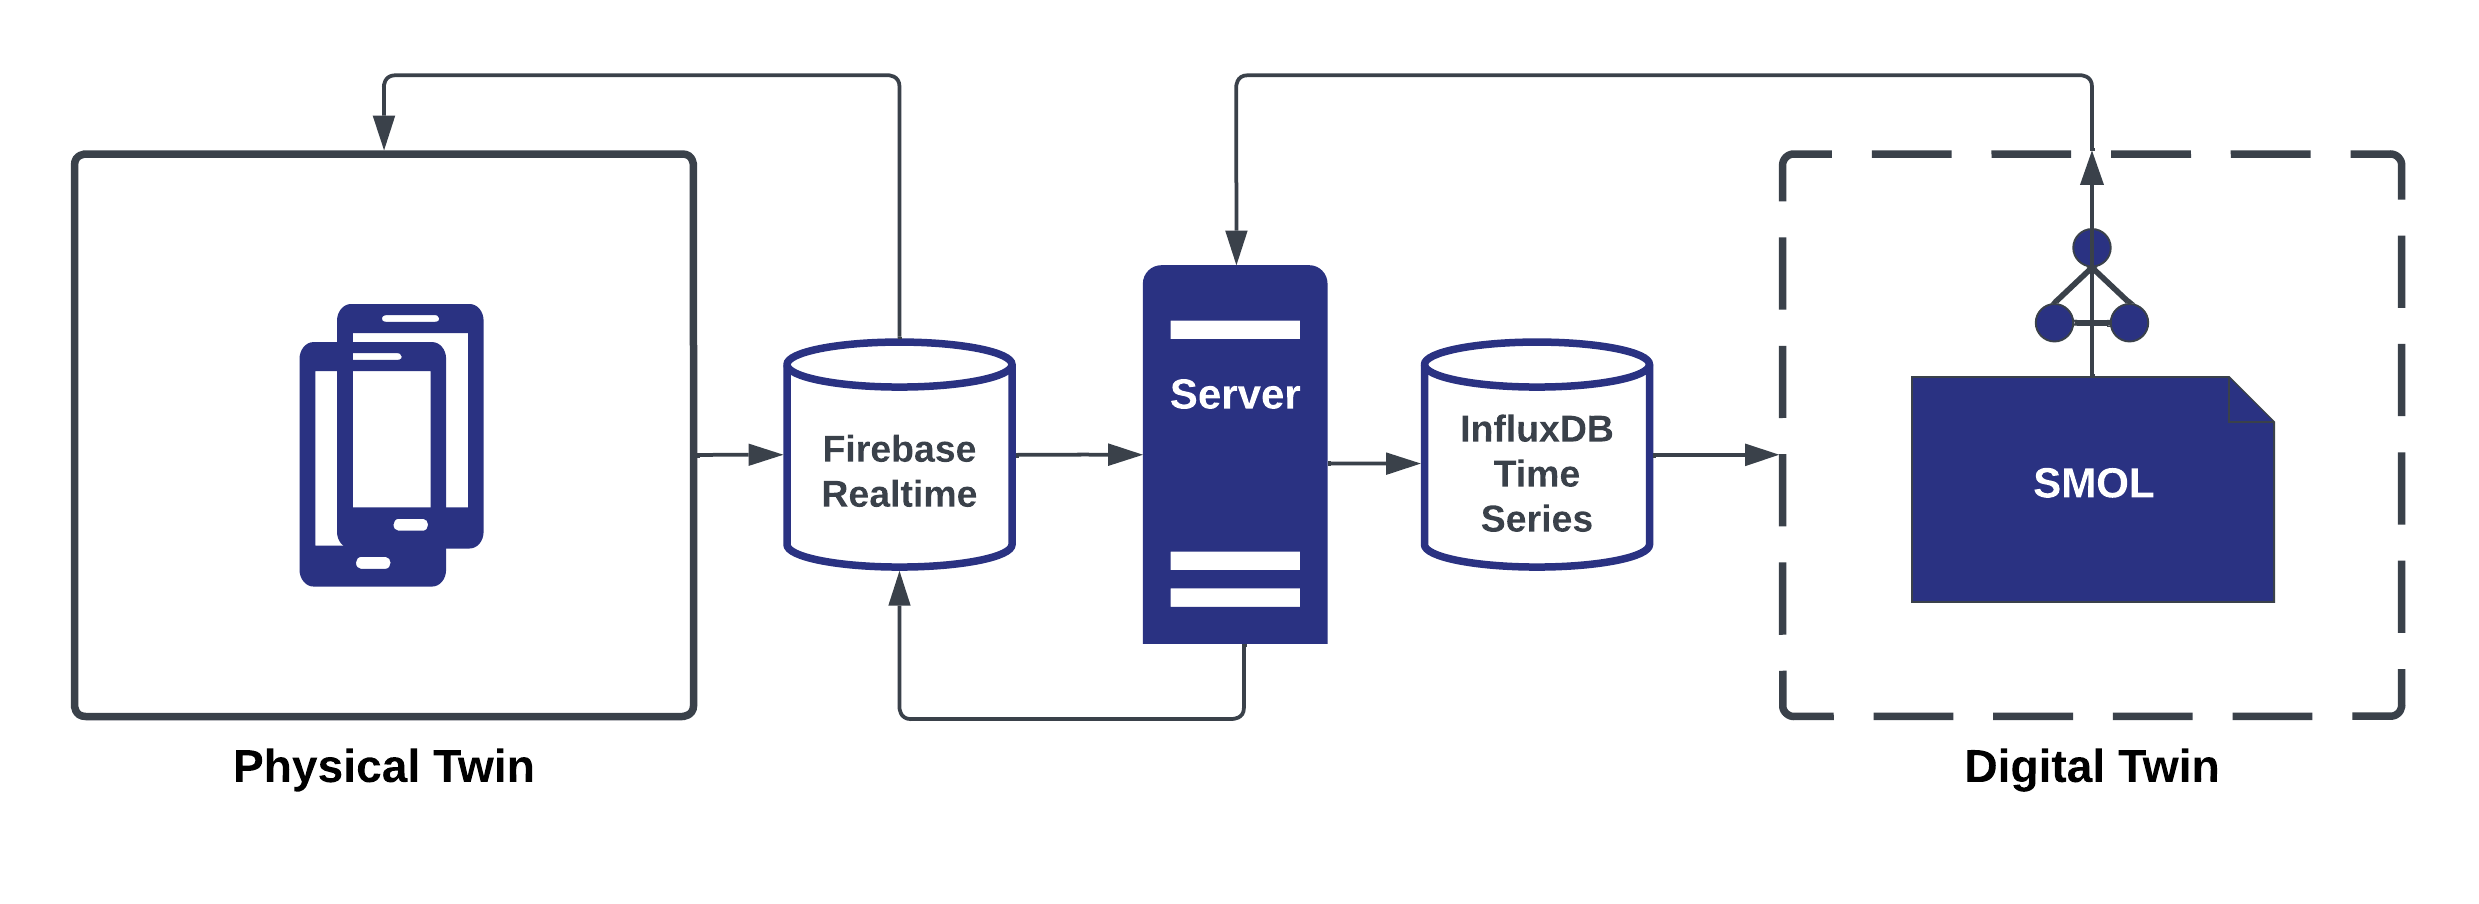
\includegraphics[scale=0.12]{graphics/thesis_overview.png}
    \caption{Overview of architectural components of the implementation in this thesis.}
    \label{fig:components}
\end{figure}

In the following sections, we describe the architectural \emph{components} in the figure one by one based on the background information and the analysis, and by referencing the corresponding \emph{part} (Client, Server, Databases, or Semantic Digital Twin) in the structural requirements.

For further reference on how we setup SMOL to be used in this thesis, see \ref{subsec:Setup}(Setup).

\subsubsection{Client}
A Flutter app was written in Dart, based on the background information on app development in industry in \ref{subsec:AppDevelopment}(Background - App Development), and from the analysis of related technologies in \ref{subsubsection:AppDevelopment}(Analysis - App Development) which describes that Flutter is popular in industry. \ref{subsec:EarlyImplementation}(Early implementation) describes the toggling of location recording in the app, but from the paragraph about GDPR (General Data Protection Regulation) in \ref{subsec:DigitalTwins} and the requirement "Ask for permission to track the physical position of the device" we implemented location permissions. The section \ref{subsec:privacy}(Privacy) discusses privacy further.

The source code of the app was structured into the following parts: 
\begin{itemize}
    \item \verb|main.dart| which initializes the app and Firebase
    \item \verb|map.dart| which contains code for the UI (User interface) in the app. This is done by rendering Flutter widgets that behave much like components in e.g. React. Simply put, the UI is what the user \emph{sees} in the app and is built from the widgets.
    \item \verb|service.dart| accesses Firebase, and writes to, or reads from it.
    \item the model-class \verb|status.dart| is used to create status objects which are sent as JSON to Firebase in which it is stored as a JSON object, as described in \ref{subsec:Databases}(Background - Databases).
\end{itemize}
We used the Google Maps SDK (Software Development Kit) in the implementation to integrate the map and its functions in the app, as described in \ref{subsec:AppDevelopment}(App Development).

Some of the requirements set forth in the structural requirements were already implemented in the earlier version of the app, such as "Client can choose to send its newest status (ID, latitude, longitude)" However, there are two requirements stating that we have to \emph{clearly} show when the recording function is off/on. In order to clearly show it for those that are color blind as well, the colors of the button changed to blue and red, respectively. Figure \ref{fig:color_theme} shows the final color theme, which is located in the previously mentioned file \verb|main.dart| and can be accessed from anywhere in the app. 

\begin{figure}[H]
    \centering
    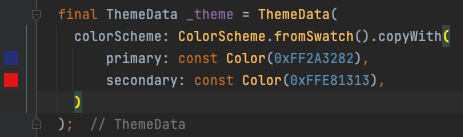
\includegraphics[scale=0.50]{graphics/color_theme.png}
    \caption{The color theme in the app.}
    \label{fig:color_theme}
\end{figure}

The Dart code in Figure \ref{fig:location_toggle} shows the rendering of the location recording button which uses the color theme above. Since the Flutter widgets are rendered and the color of the button was initially set, we had to keep track of state to change the color of the button. This was done by adding new status messages to \verb|_messages| or emptying the list in \verb|setState(() { });|. The underscore as the leading character in \verb|_messages| means that the member is only visible in its class, much like using \verb|private| for members in Java. The code also shows the use of a ternary operator, which is syntactic sugar for the conditional operators \verb|if| and \verb|else|.
\begin{figure}[H]
    \centering
    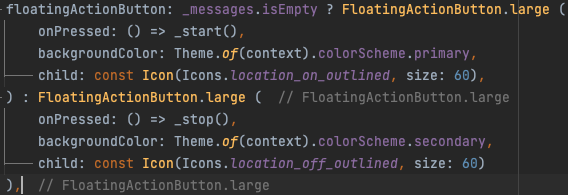
\includegraphics[scale=0.50]{graphics/location_toggle.png}
    \caption{Rendering of the location recording button in the app.}
    \label{fig:location_toggle}
\end{figure}

Furthermore, when recording of the physical location stops, the appropriate (endangered) clients are warned, as required in in the structured requirements. Firebase \emph{stores} the informed decisions, which the real-time database gets from the Digital Twin (DT) \emph{through} the server (as long as the DT has made a decision from sufficient information as analysed in \ref{subsubsec:FurtherDataSeparation}(Further data separation). Figure \ref{fig:safe_smartphone} and \ref{fig:safe_smartphone} show the conclusion of being safe and endangered, respectively.

\begin{figure}[H]
    \centering
    \begin{minipage}[c]{0.40\linewidth}
        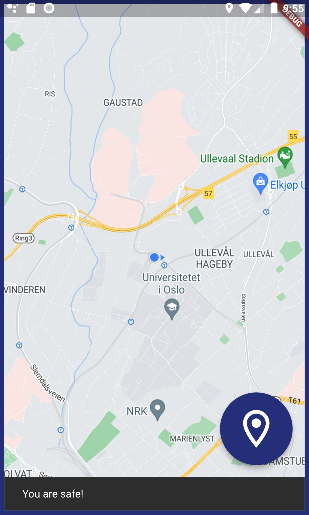
\includegraphics[width=\linewidth]{graphics/safe_smartphone.png}
        \caption{Shows that the mobile asset (smartphone) in the PT is \emph{safe} which is concluded by the DT.}
        \label{fig:safe_smartphone}
    \end{minipage}
    \hfill
    \begin{minipage}[c]{0.40\linewidth}
        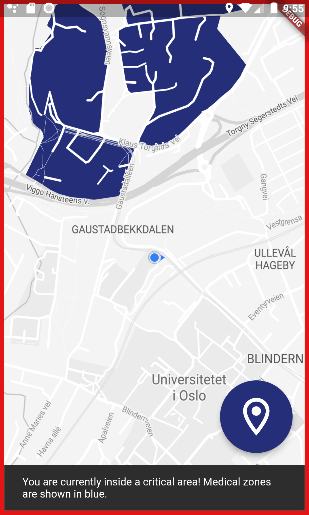
\includegraphics[width=\linewidth]{graphics/endangered_smartphone.png}
        \caption{Shows an \emph{endangered} smartphone from the informed decision to be inside a critical area, concluded by the DT.}
        \label{fig:endangered_smartphone}
    \end{minipage}
\end{figure}

\subsubsection{Server}
The main purpose of the server is full communication both ways simultaneously between the PT and the DT through the databases, which it does by using threads. Thus the server enables seamless bidirectional data flow between the PT and the DT. The \emph{items} in the \emph{server}-part in \ref{subsec:Requirements}(Structural requirements) support this. When the server runs, connections to Firebase and InfluxDB (time-series database) are setup first. Then the server forward sensor data to the DT and informed decisions to the PT simultaneously. The server prepares to send sensor data to the time-series database whenever there are new clients in the PT by keeping a reference to the list of smartphones stored in Firebase. Figure \ref{fig:insert_point} shows how a measurement point is inserted into InfluxDB. A point is made from the model-class \verb|Data|. More specifically, the instance of the \verb|Data|-class is a timestamped status message.

\begin{figure}[H]
    \centering
    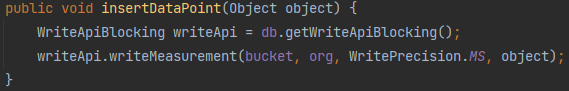
\includegraphics[scale=0.70]{graphics/insert_point.png}
    \caption{Inserting a measurement point in the Data-bucket in InfluxDB}
    \label{fig:insert_point}
\end{figure}

According to the structural requirements, the server should reload the asset model with clients that are currently tracked and access the generated knowledge graph from the DT. To reload the asset model, we used the exported OWL document (file) and put the file into the DT file structure (we later discuss how data can be stored, the reasons for using files, and the limitations to this in \ref{subsec:StoringData}(Storing data), which the server accesses and writes to using the Java framework OWL API described in \ref{subsec:Reasoning}. Based on the background information of semantic technologies in \ref{subsubsec:Technologies}, and the example of adding \textbf{individuals} of \textbf{MovableEntity} to the asset model (ontology) in \ref{subsubsec:StaticAndDynamicData}(Static and dynamic), we created a function for adding data of a smartphone to the file. Before this, we tried to use Apache Jena to reload the asset model, but it could not write data in Turtle syntax to the asset model, and we suspect some compatibility issues with the Turtle syntax in the file exported from Protégé.

Apache Jena was used to access the endangered mobile assets in the knowledge graph which was generated from a combination of the knowledge base and the state of the SMOL program in the DT. More specifically, a model of the RDF graph was loaded, and the informed decisions were forwarded to Firebase to "close the loop" of the bidirectional flow of data between the PT and the DT, as shown in Figure \ref{fig:components}.

\subsubsection{Databases}
This section shortly describes how data is stored in Firebase and InfluxDB.
In Firebase, the assigned clients are stored as unstructured nodes (JSON objects) in the list \verb|mobiles|. As discovered in the analysis of technologies in \ref{subsubsection:Databases}(Analysis - Databases), the number of nodes that can be stored are \emph{limitless}. The IDs of the endangered smartphones are also stored in a list, that is accessed by a function in \verb|service.dart| in the app. Time-series data is stored in InfluxDB in a bucket named \verb|Data|, in which there is sensor data that the SMOL program in the DT accesses. From this, the structural requirements regarding databases are met.


\subsubsection{Semantic Digital Twin}
From the background information on DTs in \ref{subsec:DigitalTwins}(Digital twins) we created a digital twin, based on a dynamic asset model of a simple building, that handled mobile assets. The DT and its parts was semantically enriched from using the semantic technologies presented in Technologies, as well as from using SMOL as an enabler of semantics from the analysis of it in \ref{subsubsec:SemanticDigitalTwins}(Semantic Digital Twins). 

The \emph{semantic} digital twin was created in SMOL by using its core language described in \ref{subsubsec:CoreLanguage}(Core Language). And by using the SMOL Interpreter (\verb|smol.jar|) in the file structure to read and execute the SMOL program. The SMOL program consists of two modular parts, namely: 
\begin{enumerate}
    \item \textbf{DS} (Digital Shadow) is a timestamped snapshot of a specific smartphone, as well as being used to access updated sensor data, from the descriptions in \ref{subsubsec:FurtherDataSeparation}.
    \item \textbf{Digital Twin} is a digital representation of the PT. It accesses: 
    \begin{enumerate}
        \item the critical areas in a building domain defined in the asset model
        \item the smartphones by their IDs from the asset model
        \item the updated physical location of the smartphones from the asset model, based on a revised version of Figure \ref{fig:access_time_series}.
    \end{enumerate}
\end{enumerate}

From this, smartphone objects are created by combining the data as shown in Figure \ref{fig:smartphone_object} by matching the IDs accessed from InfluxDB and the smartphones in the asset model. The \emph{first four requirements} in the Semantic Digital Twin-part in \ref{subsec:Requirements} are thus met. 

\begin{figure}[H]
    \centering
    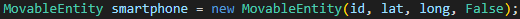
\includegraphics[scale=0.80]{graphics/smartphone_object.png}
    \caption{Creating a smartphone object by using the smartphone ID from the asset model in combination with the corresponding updated coordinates of the smartphone from InfluxDB. \textbf{False} simply means the smartphone is not concluded to be endangered yet, as this happens later on in the function in which this object is created.}
    \label{fig:smartphone_object}
\end{figure}

Referencing the requirement "Check if smartphones are inside any critical areas" we must understand what it \emph{means} before we can implement it. An example is described in \ref{subsubsec:RQ2}, where an informed decision can be made if the \emph{criteria} in the example evaluate to be true. The code implementation of it is shown in Figure \ref{fig:inside_critical_area}, where the function is located inside the Area-class. Meaning, we write \verb|area.hasPosition(lat, long)| to check if \verb|area| contains the smartphone with latitude (\verb|lat| and longitude \verb|long|).


\begin{figure}[H]
    \centering
    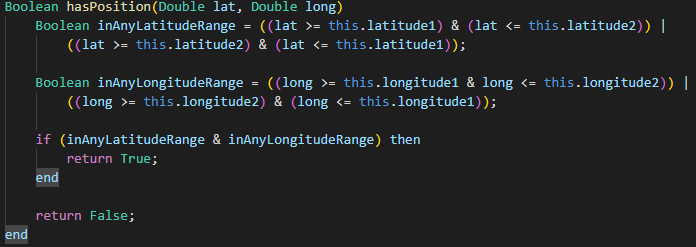
\includegraphics[scale=0.64]{graphics/inside_critical_area.png}
    \caption{Checking if a smartphone is inside a critical area based on coordinates, assuming they align.}
    \label{fig:inside_critical_area}
\end{figure}

If the DT concludes that a smartphone \emph{is} inside \emph{any} of the critical areas, the twin sets \verb|smartphone.endangered = True;| and adds the smartphone object to the specific area's list of endangered smartphones as a result, which is shown in Figure \ref{fig:add_endangered}. Note that what is shown in the figure is inside a while-loop for the context of the counter \verb|j|.

\begin{figure}[H]
    \centering
    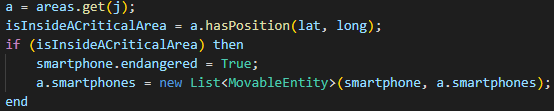
\includegraphics[scale=0.80]{graphics/add_endangered.png}
    \caption{Automatically checking if a smartphone is inside a critical area, and if it is, it is set to be endangeredm and is is added to the list of the critical area's list of endangered smartphones.}
    \label{fig:add_endangered}
\end{figure}

Regarding the last requirements of this part, informational messages, such as examples of SPARQL queries, are shown in the REPL during the program execution. Figure \ref{fig:sparql_smol} show how we can \emph{manually} manually check which smartphones are inside a critical and thus are endangered, and the results (information about endangered smartphones). The querying is done in the SMOL REPL, which is started from the information in \ref{subsubsec:SMOLInterpreter}(SMOL Interpreter).

\begin{figure}[H]
    \centering
    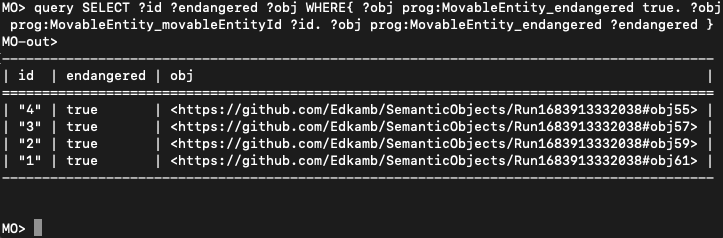
\includegraphics[scale=0.44]{graphics/sparql_smol}
    \caption{Querying with SPARQL.}
    \label{fig:sparql_smol}
\end{figure}

The DT handles newly added smartphones to the asset model that don't have a physical location as well, and thus all requirements are met.

Lastly, \ref{subsubsec:SemanticDigitalTwins} describes the use of \verb|dump| in the REPL (Read-eval-print loop) to generate the knowledge graph, which the server uses by doing the following:
\begin{enumerate}
    \item creates a \emph{model} of the knowledge graph with Apache Jena
    \item reads the model
    \item iterates over the resources (smartphones) in it
    \begin{itemize}
        \item if the smartphone is endangered, the ID of it is added to a list 
    \end{itemize}
    \item adds the list of IDs to Firebase
\end{enumerate}

Clients in the PT then access Firebase, and are warned if they are in danger from the informed decision, which closes the loop.

\newpage
\section{Evaluation}\label{sec:Evaluation}
\subsection{Setup}\label{subsec:Setup}
To setup SMOL to use in the implementation, we used \newline 
\verb|git clone https://github.com/smolang/SemanticObjects.git|
A \verb|smol.jar| file was put in the created folder at the relative file path \verb|master/twin|. Then we navigated into it with \verb|cd master/twin| and used the SMOL interpreter (\verb|smol.jar|) as described in \ref{subsubsec:SMOLInterpreter}. A good and more general guide to using SMOL is publicly available in \verb|README.md|\footnote{\url{https://github.com/smolang/SemanticObjects}}.
Comment: Overview:
setup
time it takes to make an informed decision
test runs in SMOL
   server reloads asset model
   operator adds smartphones
plotting many many smartphones with mermaid in a README.md file (url: https://github.blog/2022-02-14-include-diagrams-markdown-files-mermaid/)


\subsection{Setup of client, server and twin}
\subsection{Test runs}
\subsubsection{Server automatically reloads asset model}
\subsubsection{Operator manually updates asset model}
\subsection{Plotting with Mermaid}
\subsection{Evaluation of number of smartphones}
\subsubsection{Test with many physical devices}
\subsubsection{Results}
\subsection{How the asset model changes through time}
Evaluation of how the RDF graph produced from the asset model changes through time to show static vs dynamic data




\newpage
\section{Discussion}\label{sec:Discussion}
Comment: Look at alternatives to what is alr eady implemented, restrictions
\subsection{Storing data}\label{subsec:StoringData}
Comment: Using files and not storing RDF graphs in graph databases like other solutions (ref. Maren, Sintef papers)
Comment: Instead of updating a graph database with a knowledge graph, it is feasible to store it in the twin, as it is automatically generated by using the SMOL interpreter using the 'dump' command in the SMOL REPL and saved in a file which the server can access directly) (Should this be in Discussion?)
\subsection{Client-server communication}\label{subsec:ClientServerCommunication}
Early on we let the clients communicate with the server over TCP. This meant the IP of the server had to be known in the case of using a public network (such as at IFI) where a new IP was assigned, This meant we could only simulate using virtual device and there was a lack of support for actual physical devices devices. We looked at web sockets and FastAPI, but due to the convenience of easy integration with Firebase, came to the conclusion that Firebase Realtime Database should be used. Although another solution uses FastAPI in the architectural interconnection of its architecture (not between client and server in this case) \cite{waszak_let_2022}, Firebase was chosen because of previous experience with integrating the environment in app development. The difference between FastAPI and Firebase Realtime database in terms of performance, however, remains unclear, but as Firebase is based on websockets, it was good enough to justify using it.

\subsection{Areas}
Directions not included, instead we assume the operator knows how to create the building domain including the static building infrastructure consisting of square areas.

Comment: Reasonng with apache jena and owlapi in server, instead we just loading a model of knowledge graph with apache jena and writing to asset model with owlapi
Comment: Check if adding smartphone individuals to ontology reloads other parts of the file as well.

Comment: Can't (or shouldnt) be possible for an operator to change the dynamic parts of the asset model.



\subsection{Privacy}\label{subsec:privacy}
Comment: Privacy
    Pseudoanonymity, data is location dependant, use movement pattern to correlate data (identify data subjects) Screenshot of permission in app.
Clients get new ID's every time the physical location is recorded to deal with any privacy concerns that are left.

Comment: We use files for storing data in DT
Comment: RDFS Reasoning in server as some examples instead of just writing to and reading from asset model

Comment: However, we should keep in mind that we are creating a simple ontology. We are using HermiT because it conveniently came with the installment of Protégé. Other reasoners can be added as plugins.

Comment: Different graphs for static and dynamic data.. scales poorly and have to use graph embeddings (ref. Let the asset decide paper), although also mention that the knowledge graph is generated from the program state and from ontology where the dynamics are reflected already. Mention Neo4j as used by (cite those that use it in their implementation).

Comment: If SMOL allows us to do this… we can add the positions to the asset model from the SMOL program as well, and this way we don't have to generate the knowledge graph, and the server can instead read from the asset model, and this way we can inform the users way faster! (Can do this if time after writing the thesis). In other words, we can simply run the SMOL program, and don’t have to generate the knowledge graph by using ‘dump’ in the REPL, and so everything is fully automatic as long as the server is running…

\subsection{How data changes}
A clear separation between static and dynamic data is how often it changes through time. 

\begin{figure}
    \centering
    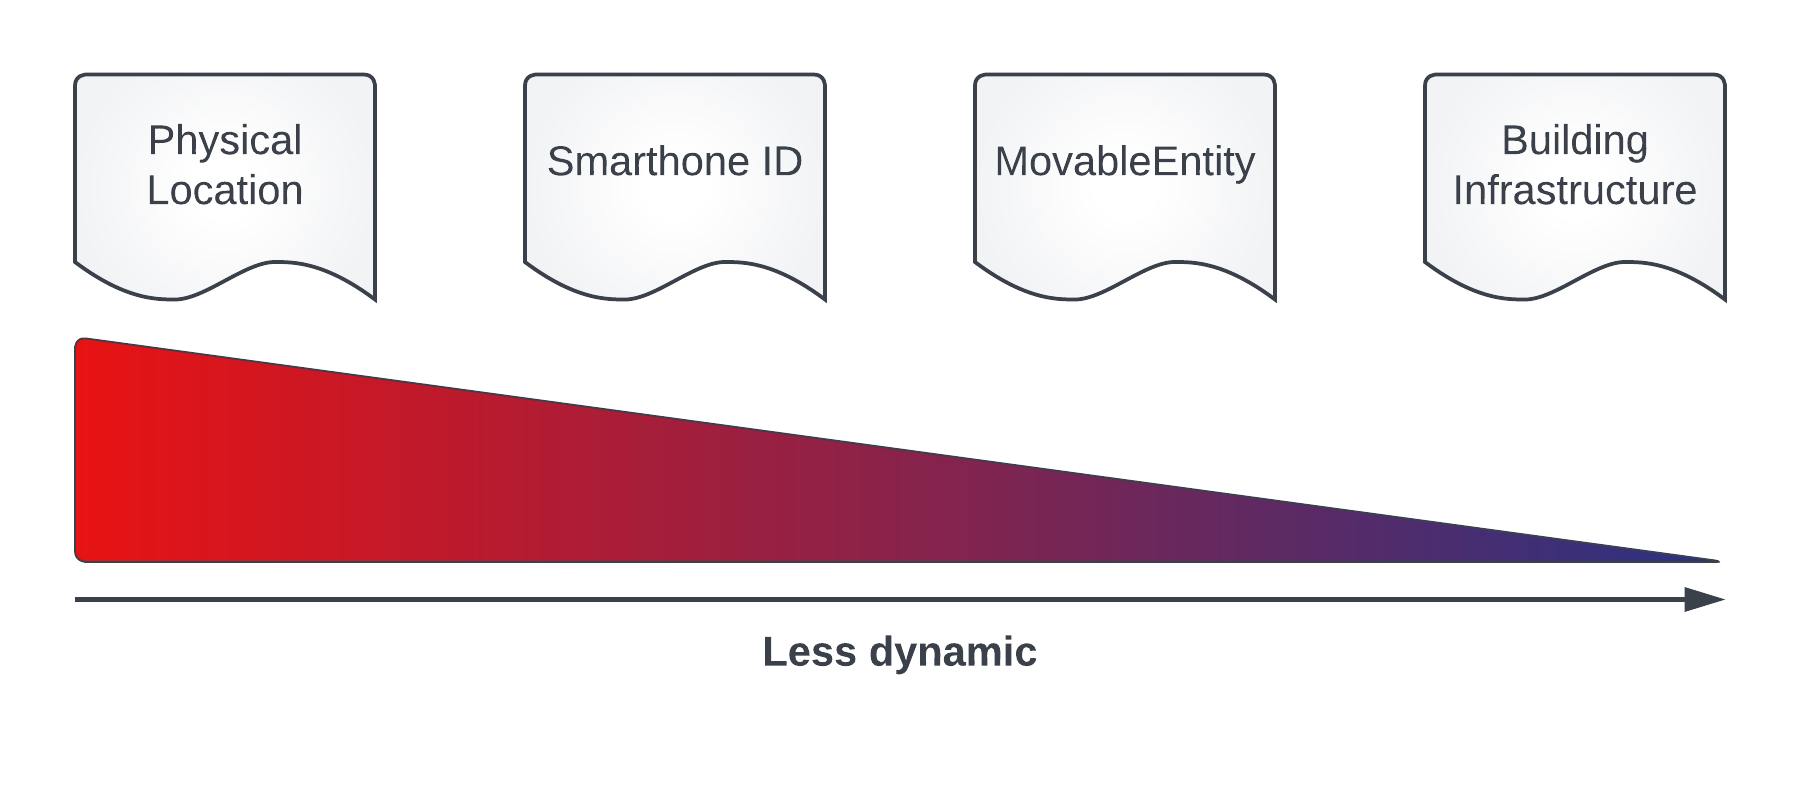
\includegraphics[scale=0.16]{graphics/dynamic_arrow.png}
    \caption{This figure shows how static and dynamic different data components are based on how often the specific data component changes through time in the implementation.}
    \label{fig:my_label}
\end{figure}


\newpage
\section{Conclusion and further work}\label{sec:Conclusion}
\subsection{Summary}
\subsection{Contributions}
Comment: DT based on a dynamic asset model, reloaded by a server, in which static and dynamic data is separated
Comment: asset model is extensible by adding newly registered smartphones and the DT takes it into account
Comment: separating static analysis of what a critical area is from the dynamic snapshots of smartphone physical locations in a digital shadow, also separated with the source code of the digital twin for modularity
\subsection{Further work}
\subsubsection{SMOL as a language under development}
Comment: Writing to Influx directly from SMOL is not possible and the time it takes to warn smartphones is limited by 'dump' to the knowledge graph.
\subsubsection{Accuracy of position}
\subsubsection{Altitude}
\subsubsection{Point-in-polygon and Mercator projection}
\subsubsection{Proximity detection}
Comment: between movable objects and static building infrastructure
\subsubsection{Anomaly detection}
Comment: \cite{li_digital_2022} mentions anomaly detections..
\subsubsection{Show mobile asset movement through time and make statistics}




\newpage
\printbibliography


\end{document}